
\clearpage
\cleardoublepage

\chapter{Experiments \& Results}

\label{chap:experiments_results}

In this chapter, we will analyze the outcomes of our extensive experimentation with various map projections and their impact on the performance
of Convolutional Neural Networks (CNNs), specifically focusing on the U-Net architecture. By systematically applying these models to various types of
map projections—cylindrical, pseudocylindrical, conic, and planar—we aim to clarify the subtle impacts these projections have on the accuracy and efficiency of
geospatial data analysis. This inquiry is rooted in a comprehensive experimental structure devised to evaluate the model's capacity to forecast precipitation patterns
from geospatial data inputs, thereby furnishing valuable insights into the optimal utilization of CNNs in the realm of geospatial analysis. Through this section,
we strive to bridge the divide between theoretical knowledge and practical implementation, making a significant contribution to the advancement of the field by
highlighting potential avenues for future research.

@TODO review [usman]
% The experimentation is conducted on four different types of map projections, namely Cylindrical, Pseudocylindrical, Conic and Planar projections.
% Then we have selected four map projections in each of the main projection types.
% The U-Net model mentioned in \autoref{chap:approach} is trained for 20 epochs for each of the map projections. Initially 120 epochs were defined for the experimentation, for each of the models the phenomenon of overfitting started to occur over the training period, to mitigate the issue \textbf{early stopping} was deployed and each model was trained for 20 epochs.
% Mean absolute error (MAE) is used as a metric for the evaluation of the model.

% 16 geospatial raster datasets with the raster resolution of 240x240 were generated for the experimentation, via the process of creating rasters as mentioned in \autoref{chap:preprocess}. The loss and the metrics discussed in the result section are the average results, as for each map projection dataset the U-Net model is trained four times mitigating the issue of randomness in the network's parameters.

% The training of the models is displayed for all of the 4 cylindrical projections and 3 of the pseudocylindrical projections, and the values of the metrics used for the evaluation of the model is displayed in a tabular form.
% For the conic and the planar projections only the evaluation metrics are shown. In the end we will discuss the overall map projections.

\section{Experimental Setup}
The experimentation is carried out on a total of four distinct types of map projections, specifically Cylindrical, Pseudocylindrical, Conic, and Planar projections.
To ensure comprehensive coverage, we have carefully chosen four map projections within each of these main projection types.

\subsection{Early Stopping}
The U-Net model, as mentioned in \autoref{chap:approach}, undergoes a training process comprising 20 epochs for each of the map projections.
Originally, a total of 120 epochs were designated for the experimentation; however, it became apparent that the phenomenon of overfitting occurred throughout the
training period for each of the models. To address this challenge, the strategy of "early stopping" was deployed, resulting in the training of each model for a reduced
duration of 20 epochs.

\subsection{Performance Evaluation}
In order to evaluate the performance of the U-Net model, the mean absolute error (MAE) is employed as a metric. This metric serves as a reliable measure to gauge
the accuracy and precision of the model's predictions.
\subsection{Raster Generation}
Furthermore, a set of 16 geospatial raster datasets, each with a raster resolution of 240x240, were generated specifically for the purpose of this experimentation.
These datasets were created using the raster creation process detailed in \autoref{chap:preprocess}. It is important to note that the reported loss and metrics discussed
in the results section represent average values. This is due to the fact that for each map projection dataset, the U-Net model is trained four times, thereby mitigating
the potential impact of random variations in the network's parameters.
\subsection{Model Training Analysis}
The training progress of the models is meticulously documented for all four cylindrical projections, as well of the pseudocylindrical projections.
Additionally, the values of the evaluation metrics employed to assess the model's performance are presented in a concise tabular format.

However, for the conic and planar projections, only the evaluation metrics are showcased as these particular projections do not undergo the same level of detailed training
analysis.

Finally, following the presentation of the specific experimental results, a comprehensive discussion will be conducted to provide an overarching analysis of the
various map projections under consideration.

\clearpage

\section{Cylindrical Projections}

The four cylindrical map projections used for the experimentation are
\begin{itemize}
    \item Mercator
    \item Plate Carree
    \item Cylindrical Equal Area
    \item General Oblique Transformation
\end{itemize}
The selection of the map projections is done based on the underlying properties of the cylindrical map projections mentioned in the \autoref{section:map_projections}. These projections try to mitigate some of the underlying distortions generated by the projections.

\subsection{Mercator}
\begin{figure}[H]
    \centering
    \begin{minipage}{0.30\textwidth}
        \centering
        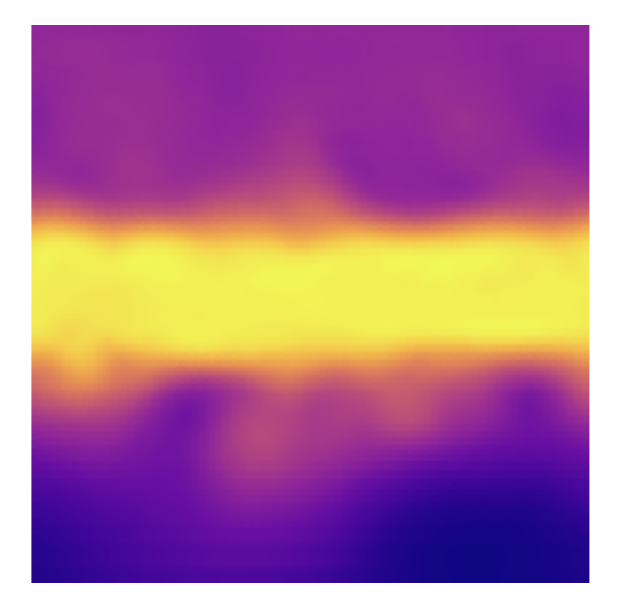
\includegraphics[width=0.9\linewidth]{figures/chapter-8/geopoth_mercator.png}
        \caption{ Geopotential height raster data as Mercator projected}
        \label{fig:merc_geopoth_raster}
    \end{minipage}\hfill
    \begin{minipage}{0.30\textwidth}
        \centering
        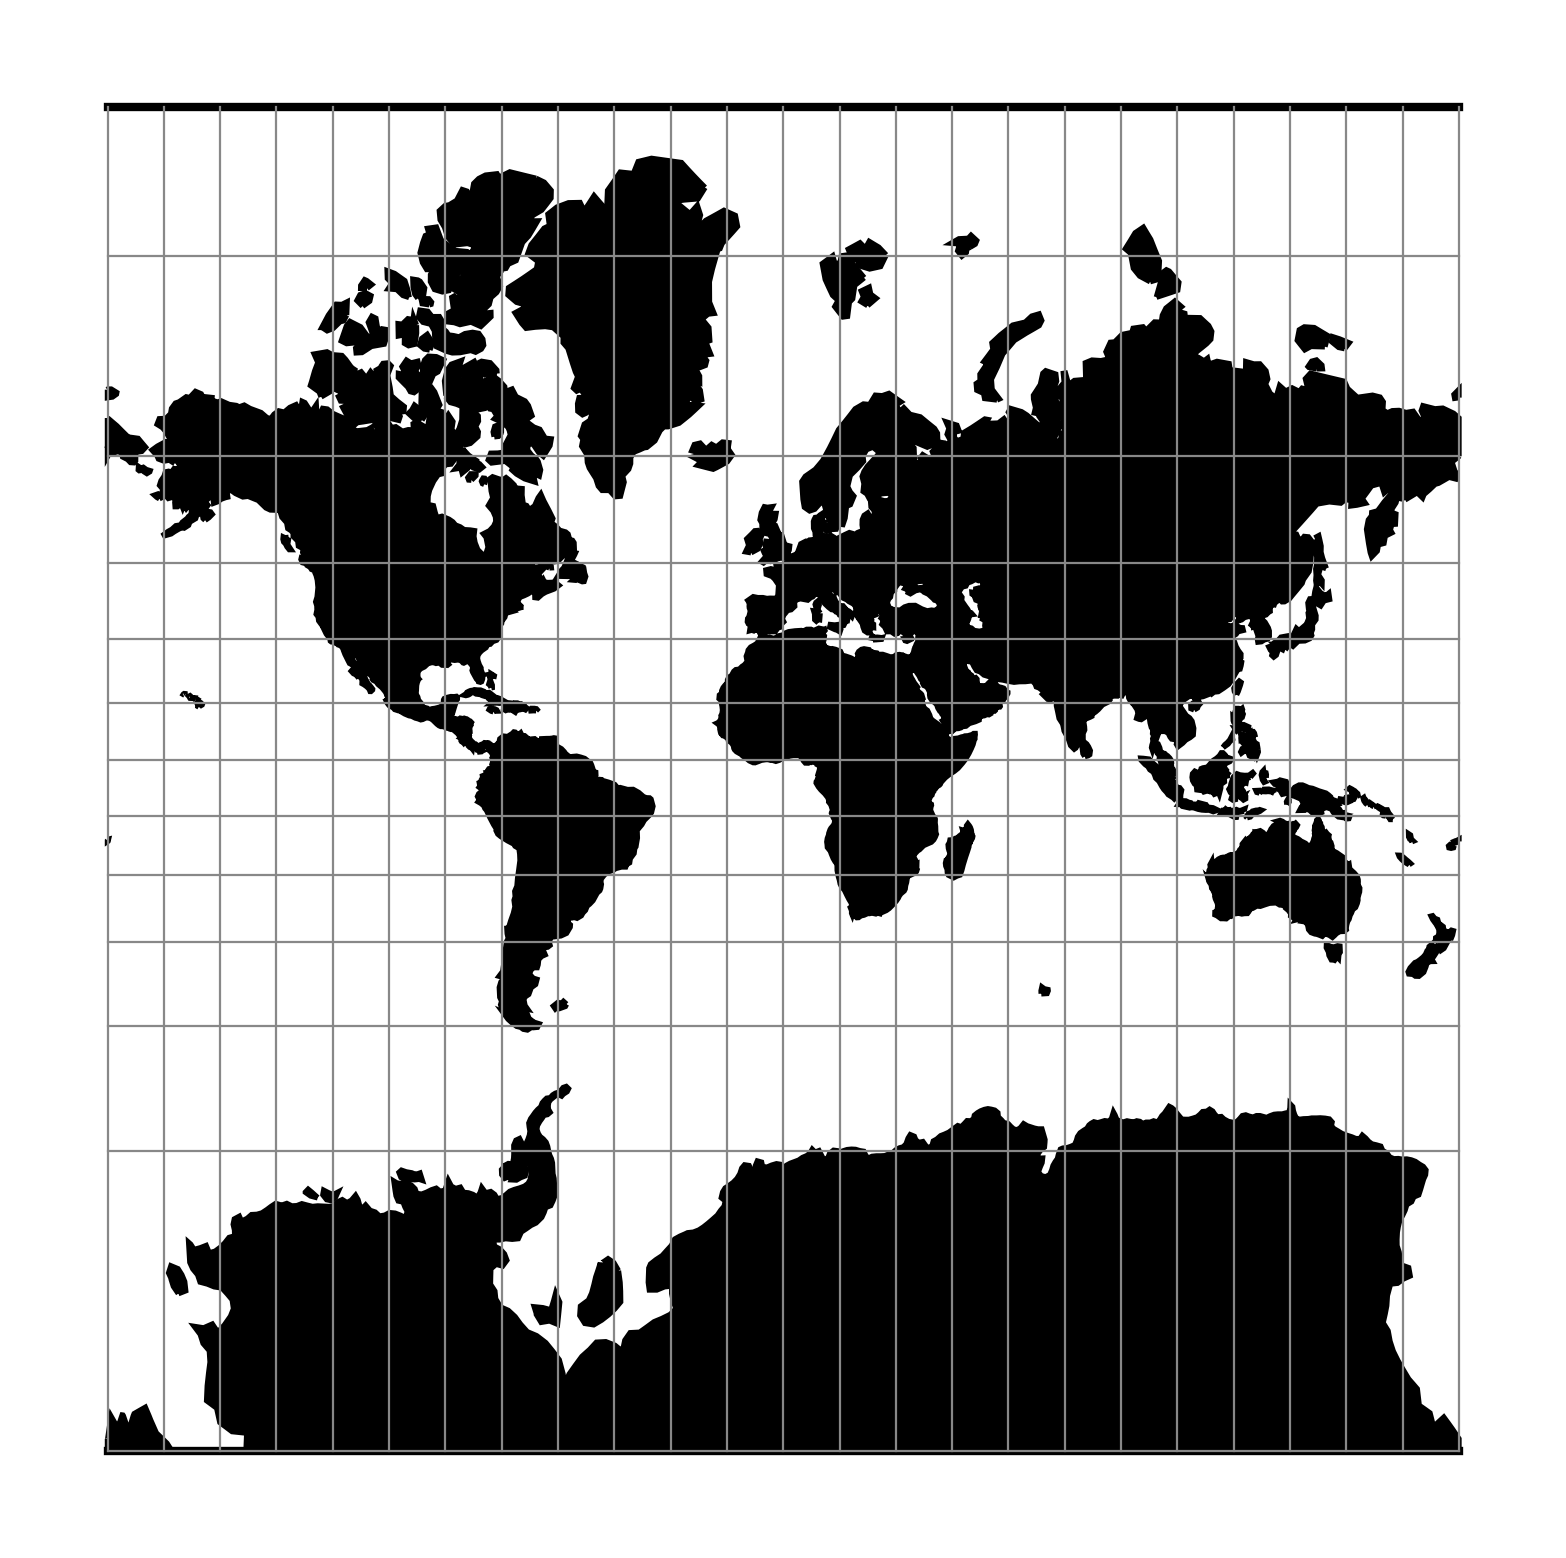
\includegraphics[width=0.9\linewidth]{figures/chapter-8/merc.png}
        \caption{Mercator Projection (Source \cite{PROJ_SITE})}
        \label{fig:merc_proj}
    \end{minipage}\hfill
    \begin{minipage}{0.30\textwidth}
        \centering
        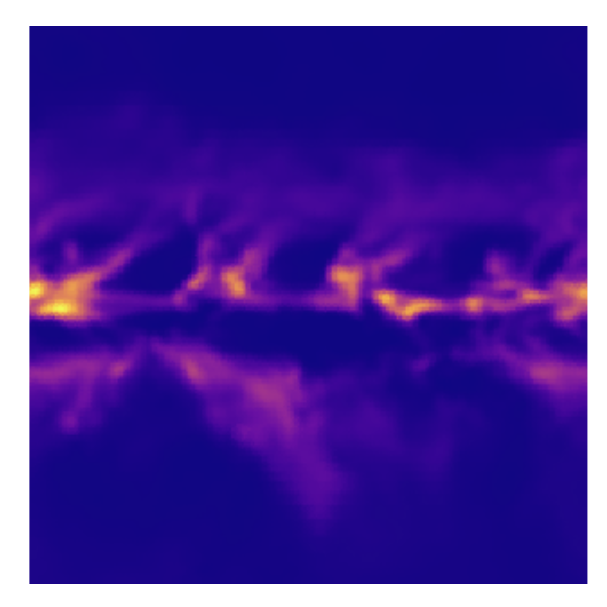
\includegraphics[width=0.9\linewidth]{figures/chapter-8/prect_mercator.png}
        \caption{Precipitation raster data as Mercator projected}
        \label{fig:merc_prect_raster}
    \end{minipage}\hfill
\end{figure}

\begin{figure}[H]
    \centering
    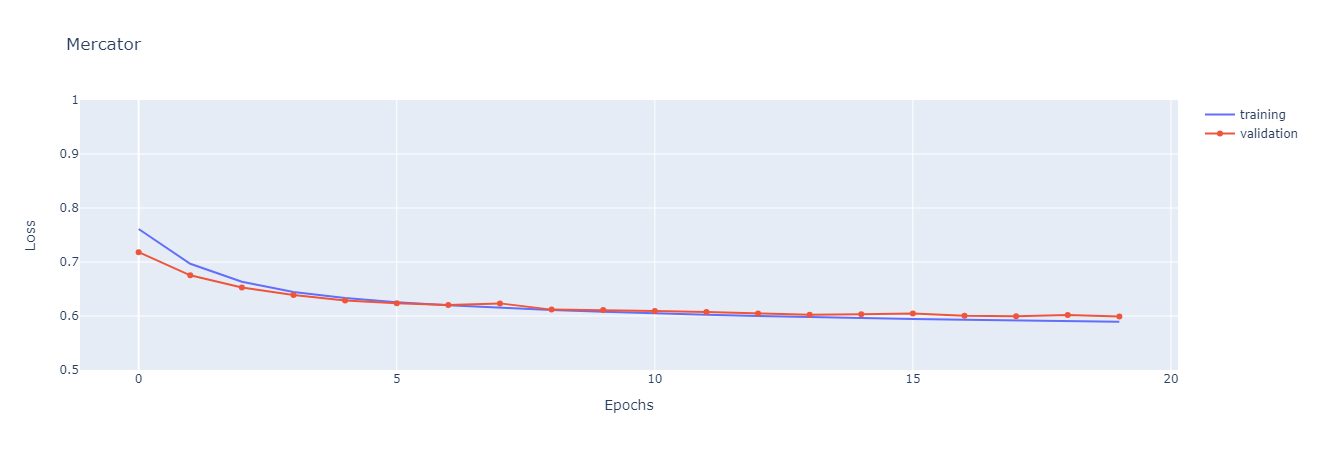
\includegraphics[width=1.0\linewidth]{figures/chapter-8/merc_loss.png}
    \caption{Mercator: Averaged training loss of models  }
    \label{fig:merc_loss}
\end{figure}

\newpage

\subsection{Plate Carree}

\begin{figure}[H]
    \centering
    \begin{minipage}{0.30\textwidth}
        \centering
        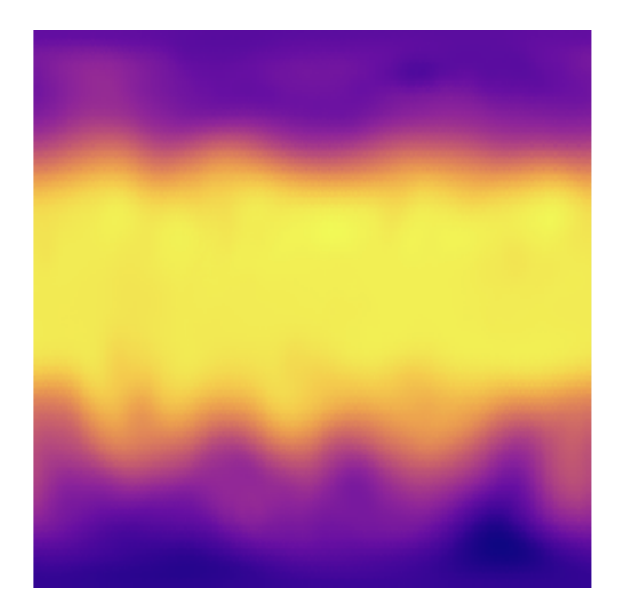
\includegraphics[width=0.9\linewidth]{figures/chapter-8/plate_caree_geopoth_raster.png}
        \caption{ Geopotential height raster data as Plate Carree projected}
        \label{fig:eqc_geopoth_raster}
    \end{minipage}\hfill
    \begin{minipage}{0.30\textwidth}
        \centering
        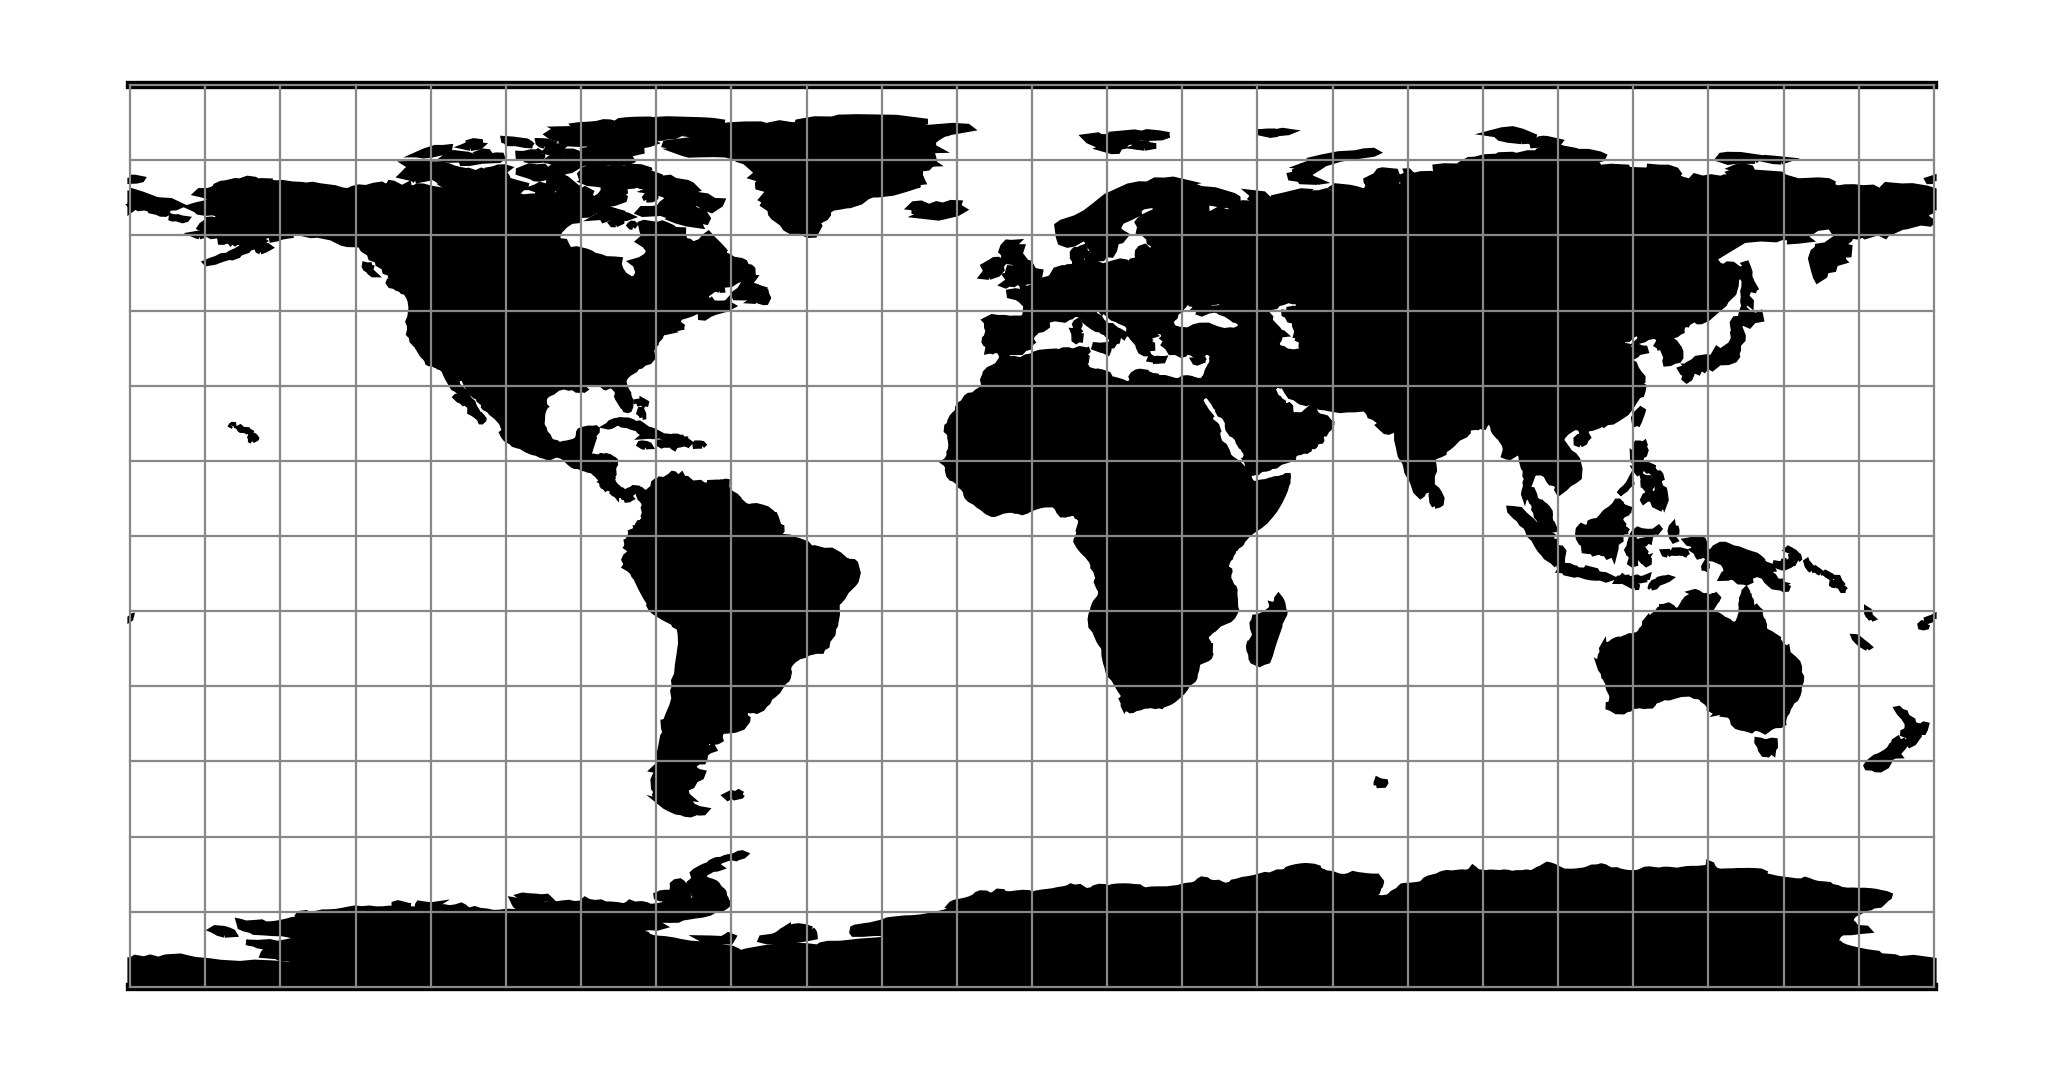
\includegraphics[width=0.9\linewidth]{figures/chapter-8/eqc.png}
        \caption{Plate Carree Projection (Source \cite{PROJ_SITE})}
        \label{fig:eqc_prect_raster}
    \end{minipage}\hfill
    \begin{minipage}{0.30\textwidth}
        \centering
        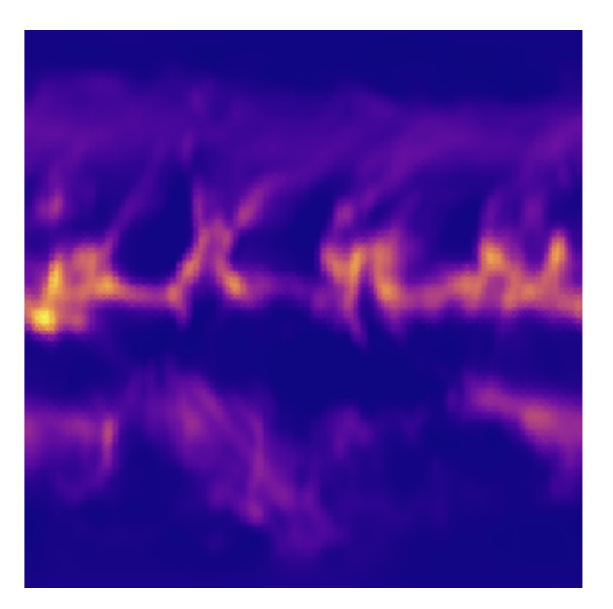
\includegraphics[width=0.9\linewidth]{figures/chapter-8/plate_caree_prect_raster.png}
        \caption{Precipitation raster data as Plate Carree projected}
        \label{fig:eqc_prect_raster}
    \end{minipage}\hfill
\end{figure}

\begin{figure}[H]
    \centering
    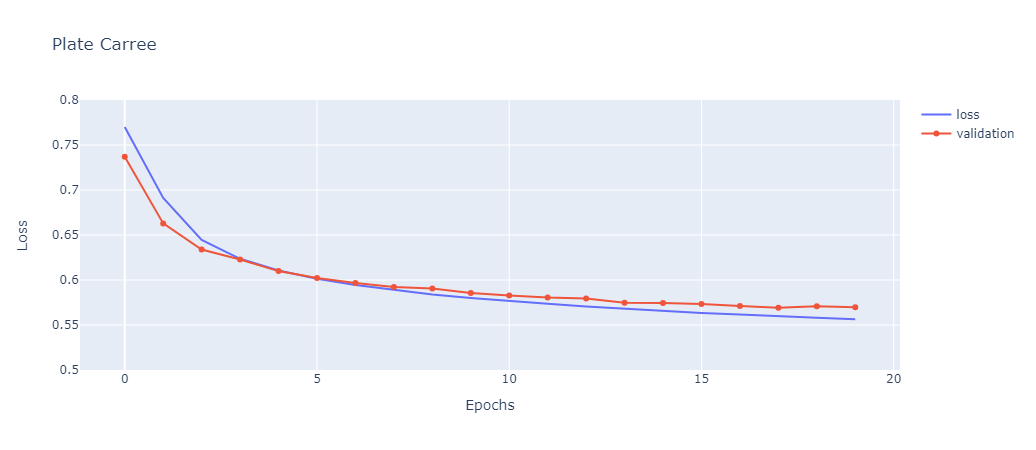
\includegraphics[width=1.0\linewidth]{figures/chapter-8/pc_loss.png}
    \caption{Plate Carree: Averaged training loss of models  }
    \label{fig:pc_loss}
\end{figure}

The trend for the training of the model


\subsection{Cylindrical Equal Area}

\begin{figure}[H]
    \centering
    \begin{minipage}{0.30\textwidth}
        \centering
        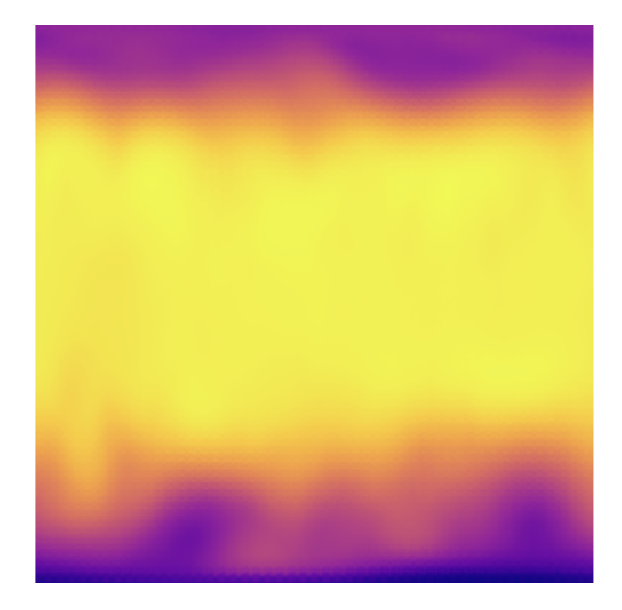
\includegraphics[width=0.9\linewidth]{figures/chapter-8/prect_cea.png}
        \caption{ Geopotential height raster data as Cylindrical Equal Area projected}
        \label{fig:cea_geopoth_raster}
    \end{minipage}\hfill
    \begin{minipage}{0.30\textwidth}
        \centering
        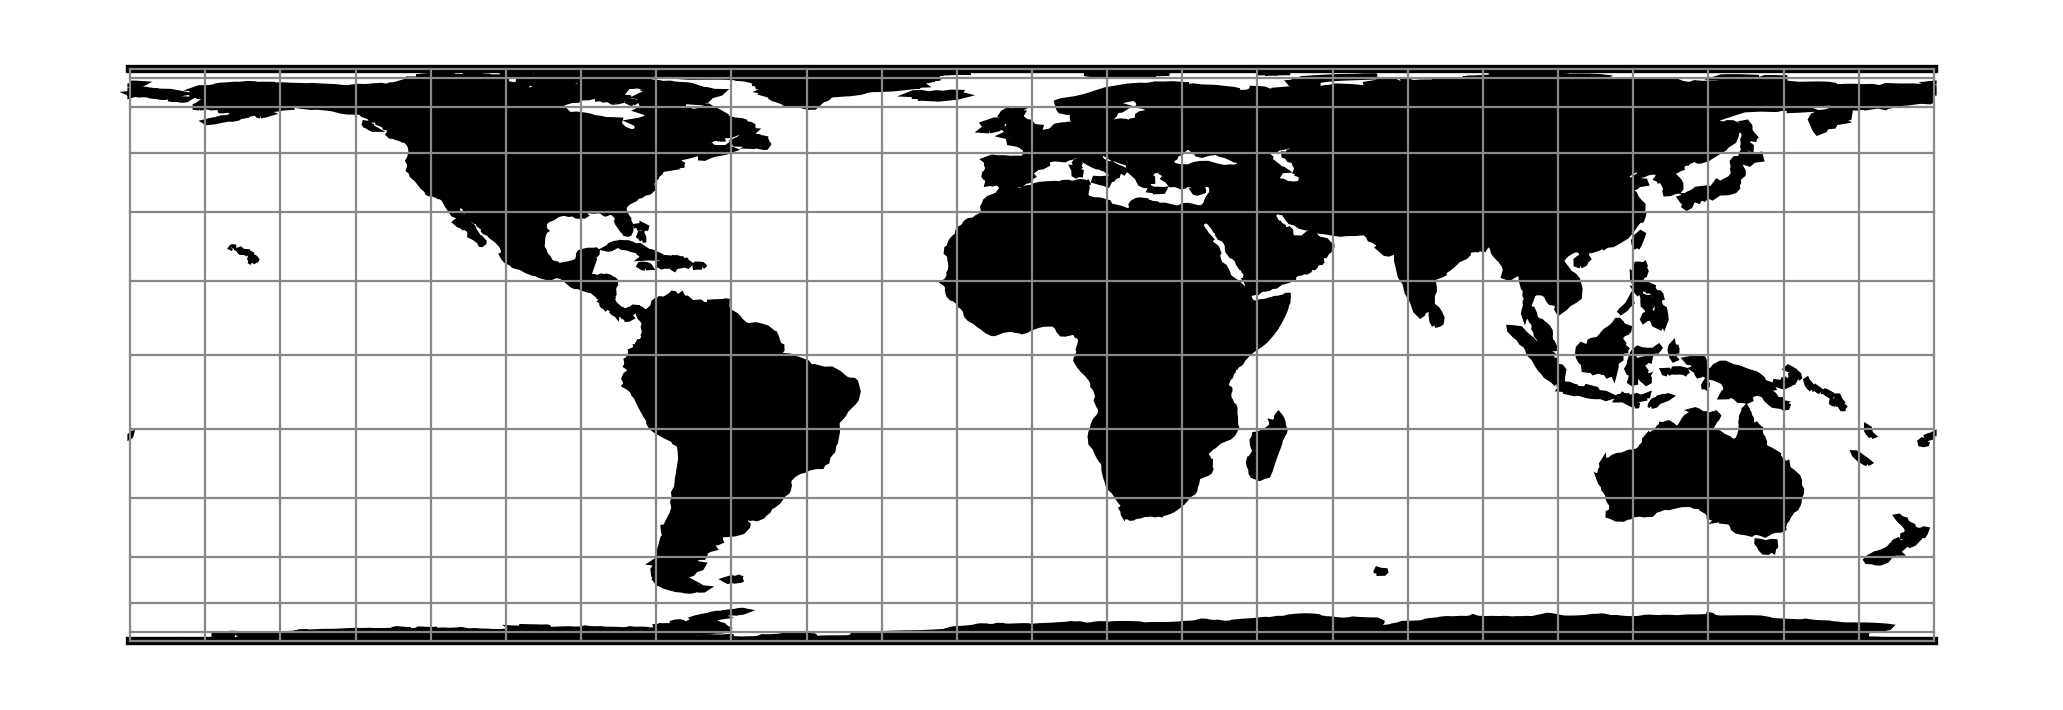
\includegraphics[width=0.9\linewidth]{figures/chapter-8/cea.png}
        \caption{Cylindrical Equal Area Projection (Source \cite{PROJ_SITE})}
        \label{fig:cea_prect_raster}
    \end{minipage}\hfill
    \begin{minipage}{0.30\textwidth}
        \centering
        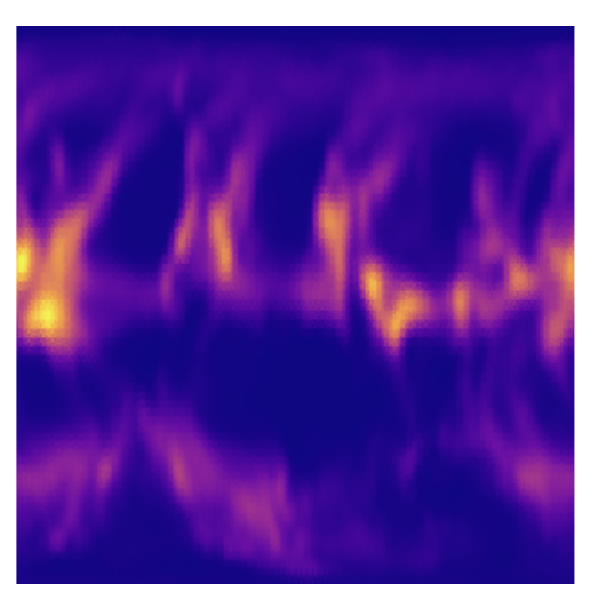
\includegraphics[width=0.9\linewidth]{figures/chapter-8/geopoth_cea.png}
        \caption{Precipitation raster data as Cylindrical Equal Area projected}
        \label{fig:cea_prect_raster}
    \end{minipage}\hfill
\end{figure}

\begin{figure}[h]
    \centering
    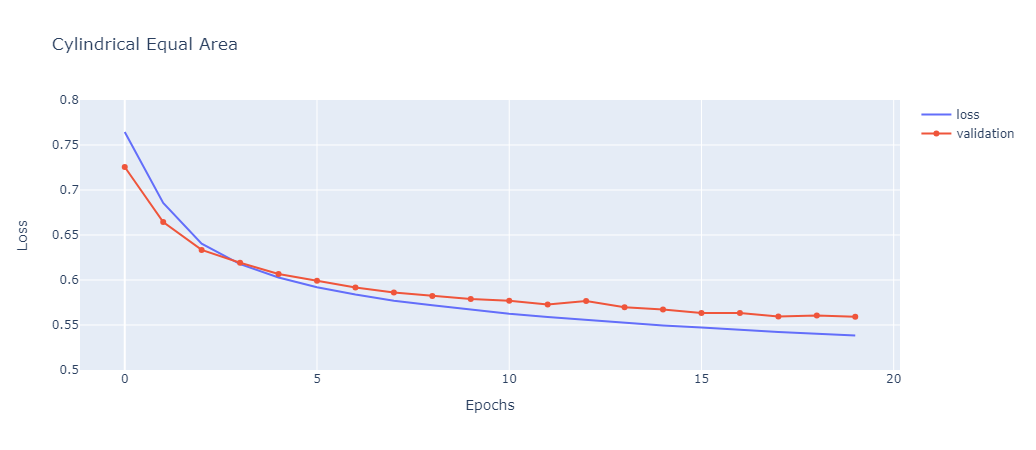
\includegraphics[width=1.0\linewidth]{figures/chapter-8/cea_loss.png}
    \caption{Cylindrical Equal Area: Averaged training loss of models  }
    \label{fig:cea_loss}
\end{figure}

\subsection{General Oblique Transformation}
\begin{figure}[H]
    \centering
    \begin{minipage}{0.30\textwidth}
        \centering
        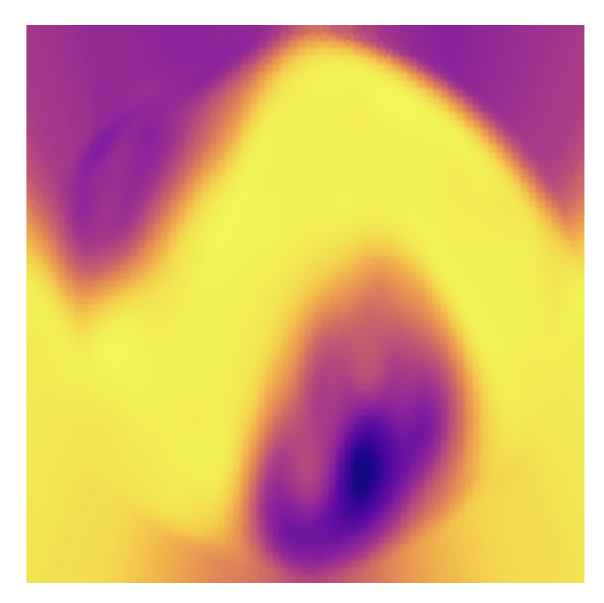
\includegraphics[width=0.9\linewidth]{figures/chapter-8/geopoth_got.png}
        \caption{ Geopotential height raster data as General Oblique Transformation projected}
        \label{fig:ob_tran_geopoth_raster}
    \end{minipage}\hfill
    \begin{minipage}{0.30\textwidth}
        \centering
        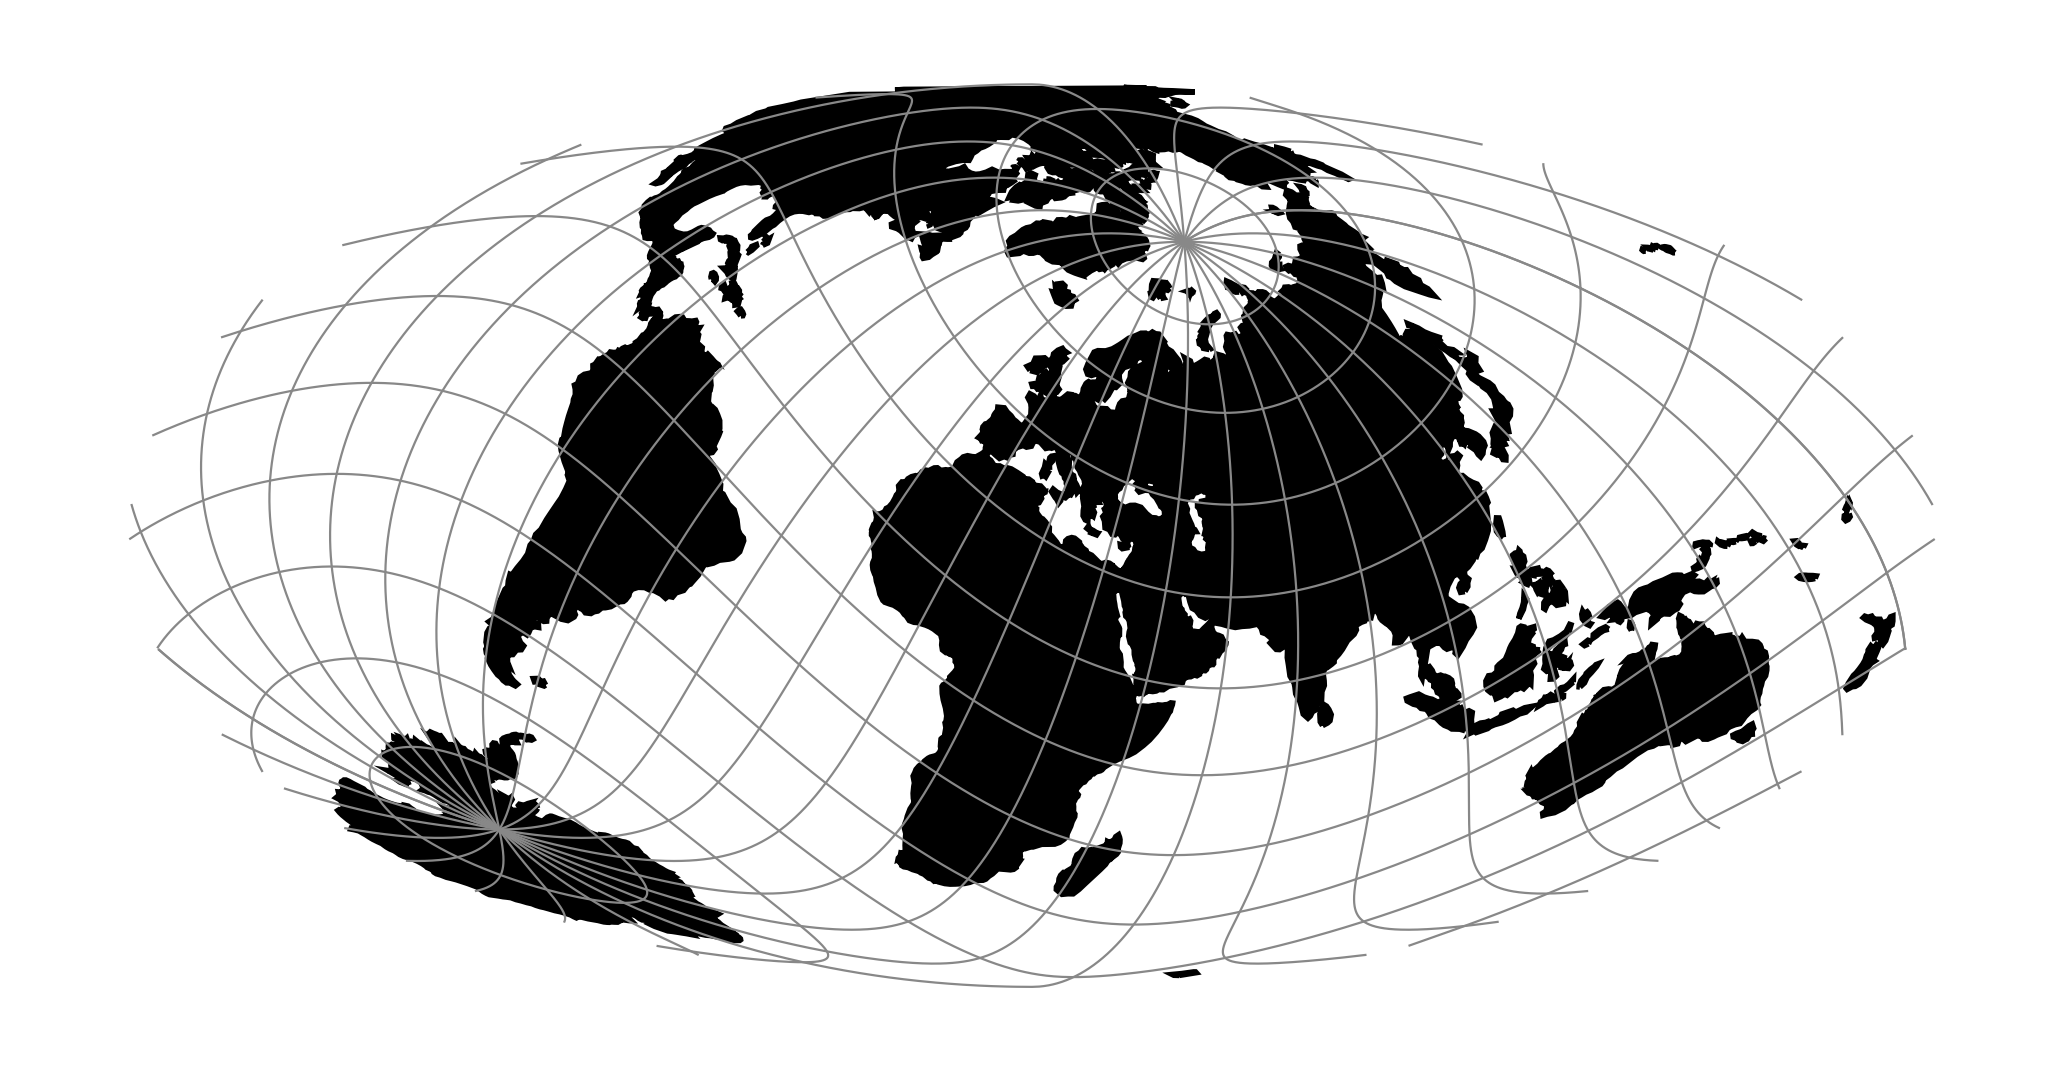
\includegraphics[width=0.9\linewidth]{figures/chapter-8/ob_tran.png}
        \caption{General Oblique Transformation Projection (Source \cite{PROJ_SITE})}
        \label{fig:ob_tran_proj}
    \end{minipage}\hfill
    \begin{minipage}{0.30\textwidth}
        \centering
        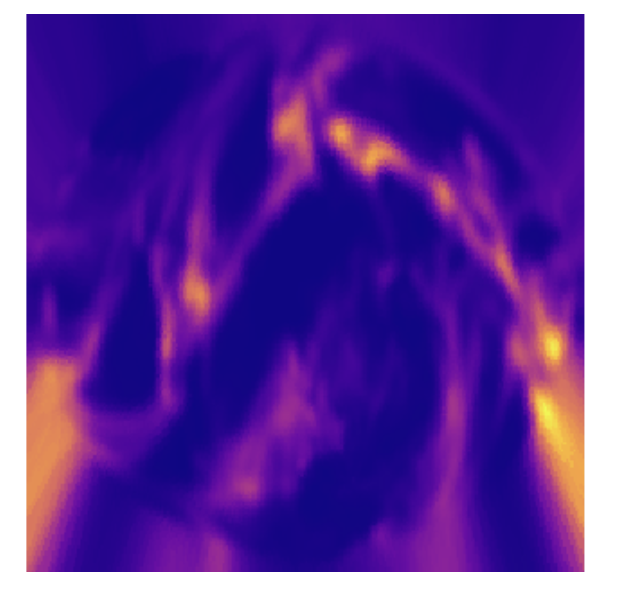
\includegraphics[width=0.9\linewidth]{figures/chapter-8/prect_got.png}
        \caption{Precipitation raster data as General Oblique Transformation projected}
        \label{fig:ob_tran_prect_raster}
    \end{minipage}\hfill
\end{figure}

\begin{figure}[H]
    \centering
    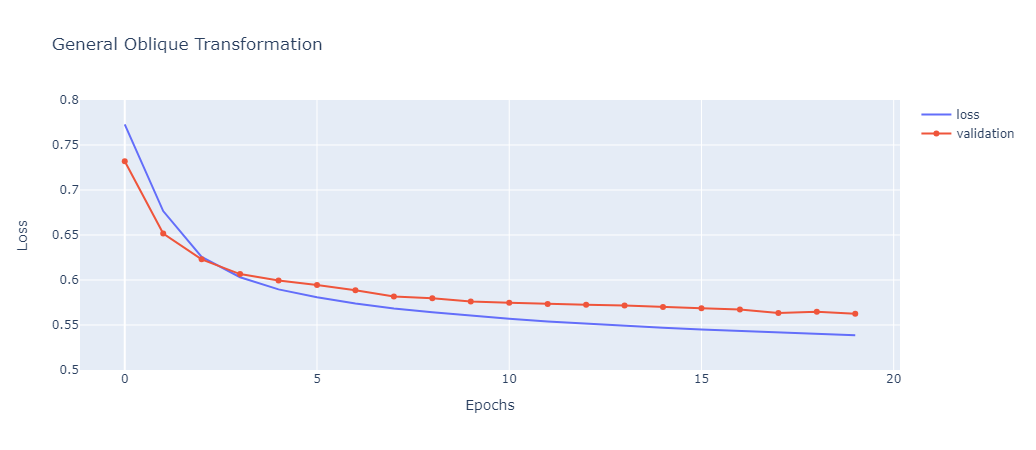
\includegraphics[width=1.0\linewidth]{figures/chapter-8/got_loss.png}
    \caption{General Oblique Transformation: Averaged training loss of models  }
    \label{fig:got_loss}
\end{figure}
\subsection{Results \& Observations}
\begin{itemize}
    \item The ~\ref{fig:merc_loss} shows the average training loss for the U-Net model mentioned in the \autoref{chap:approach}, it could be seen that model's training loss is stabalizing and the trend of the validation loss is on a decrease.
          The model is being trained well for the Mercator projection, we need to consider the fact that we have trained a shallow model with less numbers of filters.
    \item The ~\ref{fig:pc_loss} shows the average training loss decreasing and the trend of the validation loss is on an increase after the 17th epoch, with more training the model is on the path to overfit. Early stopping should have been used earlier for this projection dataset.
    \item ~\ref{fig:cea_loss} depicts that the model in training is subjected to overfit very quickly in the training process. Just after the 7th epoch the model is overfitting.
    \item ~\ref{fig:got_loss} shows, the model start to overfit from the 5th epoch.
    \item As soon as the rasters which are generated to resolve some of the distortions occuring due to map projections the rasters.
          The cylindrical equal area projection does resolve the distortion of area but is not able to perform well during the training of the model under observation.
          Same is the case with oblique general transformation projection, as it brings the north polar region at the central level part, but brings huge distortions equator regions.
    \item In our case the input data to the model, geopotential height when subjected to the whole raster, the model in under consideration tends to overfit.
    \item The ~\ref{cylindrical_results_table} depicts the MAE to measure the quality of the predictions of the precipitation on the average results.

\end{itemize}
\begin{table}[ht]
    \centering
    \caption{Summary of Cylindrical Projection Model Performance}
    \label{cylindrical_results_table}
    \renewcommand{\arraystretch}{1.2} % Adjusts the row height
    \begin{tabular}{|l|c|c|c|c|c|}
        \hline
        \rowcolor[gray]{0.9}
        \textbf{\emph{Project Name}}   & \textbf{\emph{Epochs}} & \textbf{\emph{MAE}} & \textbf{\emph{Validation MAE}} \\ \hline
        Mercator                       & 20                     & 0.51                & 0.51                           \\ \hline
        Plate Carree                   & 20                     & 0.49                & 0.49                           \\ \hline
        Cylindrical Equal Area         & 20                     & 0.48                & 0.49                           \\ \hline
        General Oblique Transformation & 20                     & 0.48                & 0.49                           \\ \hline
    \end{tabular}


\end{table}
\clearpage
\newpage

\section{Experiments: Pseudocylindrical projections}
The selected pseudocylindrical projections for the experimentation are mentioned below:
\begin{itemize}
    \item Robinson
    \item Interrupted Goode Homolosine
    \item Sinusoidal (Sanson Flamsteed)
    \item Loximuthal
\end{itemize}
\subsection{Robinson}
\begin{figure}[H]
    \centering
    \begin{minipage}{0.30\textwidth}
        \centering
        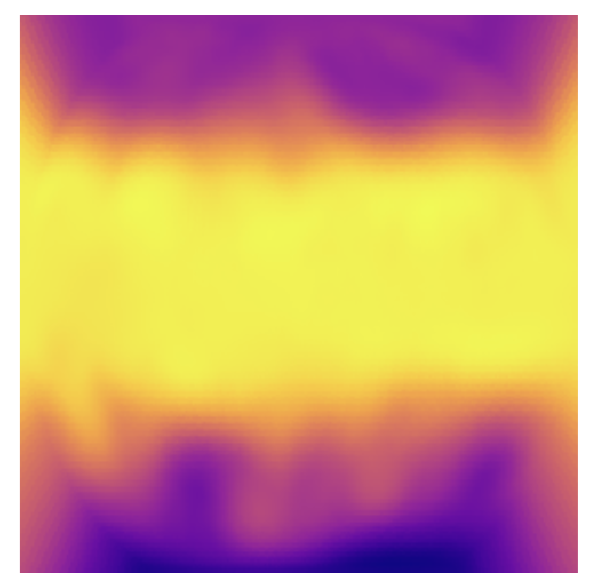
\includegraphics[width=0.9\linewidth]{figures/chapter-8/geopoth_robin.png}
        \caption{ Geopotential height raster data as Robinson projected}
        \label{fig:robin_geopoth_raster}
    \end{minipage}\hfill
    \begin{minipage}{0.30\textwidth}
        \centering
        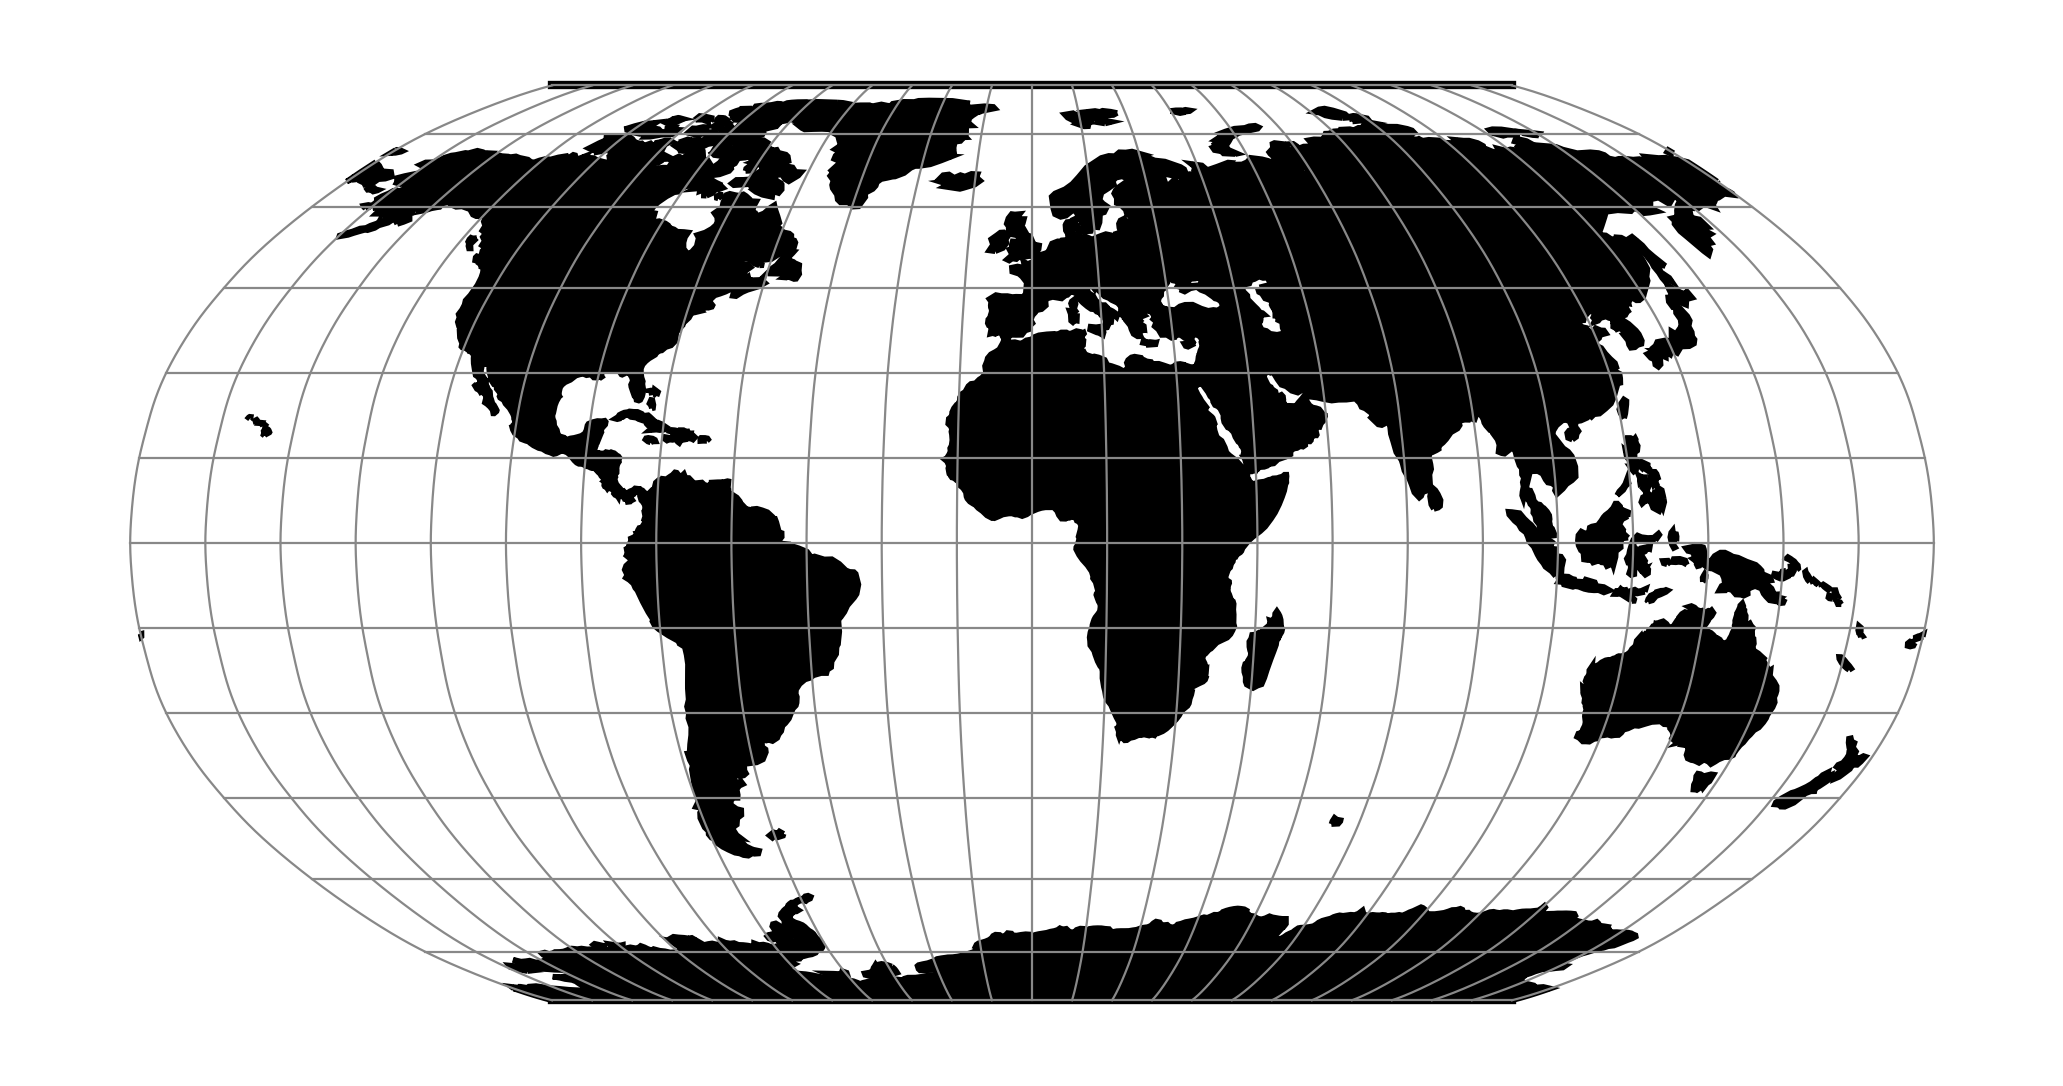
\includegraphics[width=0.9\linewidth]{figures/chapter-8/robin.png}
        \caption{Robinson (Source \cite{PROJ_SITE})}
        \label{fig:robin_proj}
    \end{minipage}\hfill
    \begin{minipage}{0.30\textwidth}
        \centering
        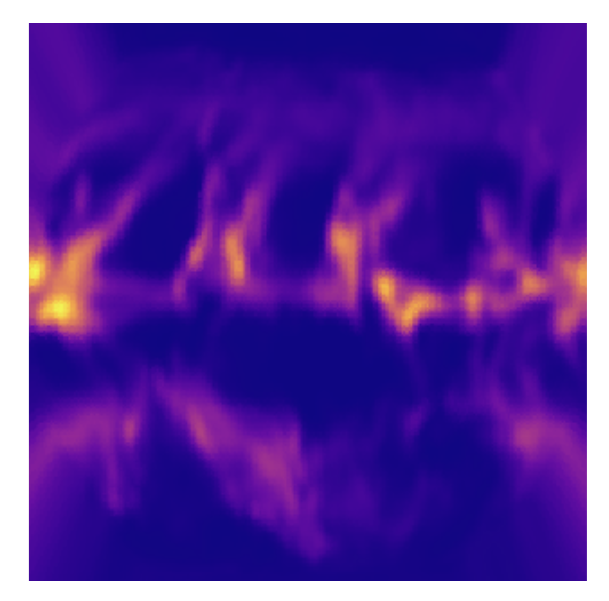
\includegraphics[width=0.9\linewidth]{figures/chapter-8/prect_robin.png}
        \caption{Precipitation raster data as Robinson projected}
        \label{fig:robin_prect_raster}
    \end{minipage}\hfill
\end{figure}
\begin{figure}[H]
    \centering
    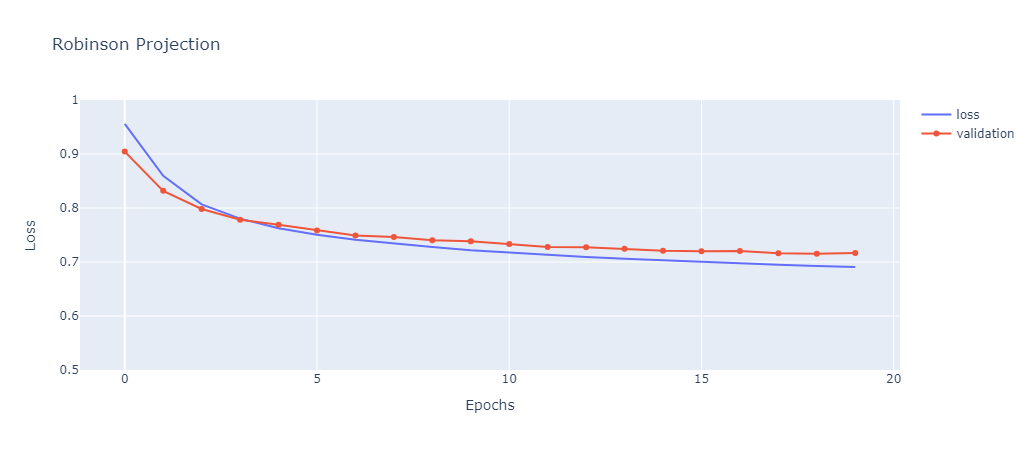
\includegraphics[width=1.0\linewidth]{figures/chapter-8/robin_loss.png}
    \caption{Robinson: Averaged training loss of models  }
    \label{fig:robin_loss}
\end{figure}
\subsection{Interrupted Goode Homolosine}
\begin{figure}[H]
    \centering
    \begin{minipage}{0.30\textwidth}
        \centering
        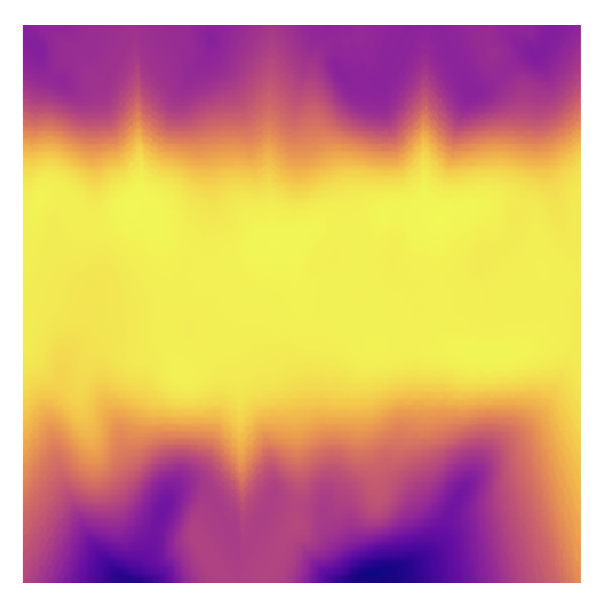
\includegraphics[width=0.9\linewidth]{figures/chapter-8/geopoth_goode.png}
        \caption{ Geopotential height raster data as Interrupted Goode Homolosine projected}
        \label{fig:ig_geopoth_raster}
    \end{minipage}\hfill
    \begin{minipage}{0.30\textwidth}
        \centering
        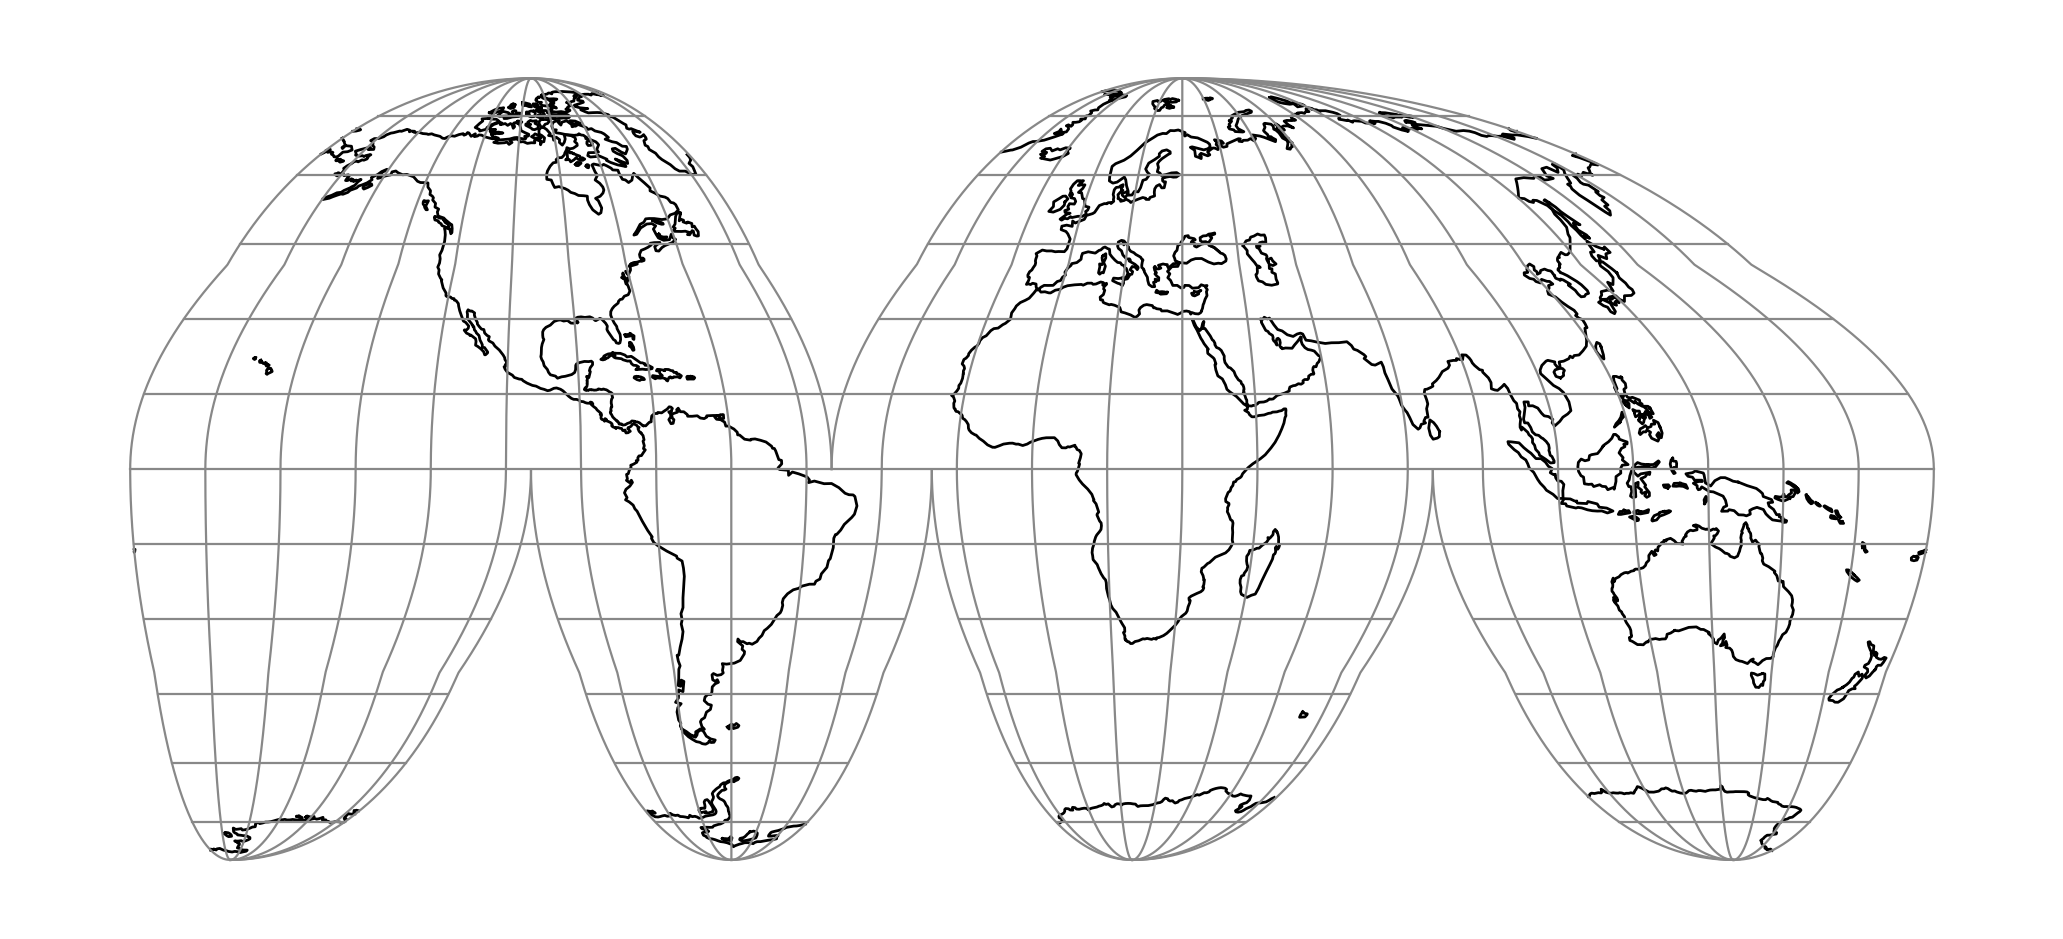
\includegraphics[width=0.9\linewidth]{figures/chapter-8/igh.png}
        \caption{Interrupted Goode Homolosine (Source \cite{PROJ_SITE})}
        \label{fig:ig_proj}
    \end{minipage}\hfill
    \begin{minipage}{0.30\textwidth}
        \centering
        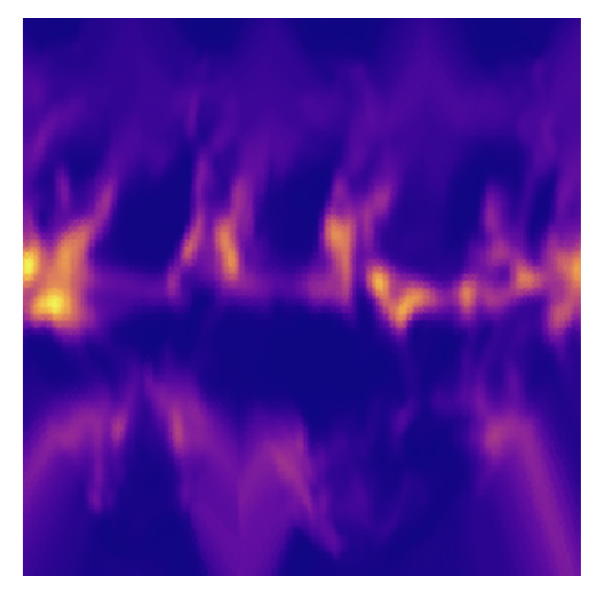
\includegraphics[width=0.9\linewidth]{figures/chapter-8/prect_goode.png}
        \caption{Precipitation raster data as Interrupted Goode Homolosine projected}
        \label{fig:ig_prect_raster}
    \end{minipage}\hfill
\end{figure}

\begin{figure}[H]
    \centering
    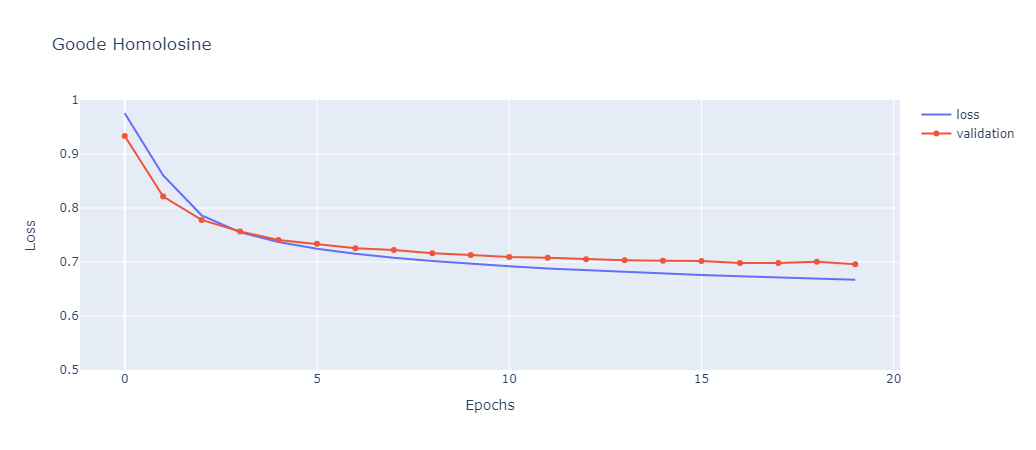
\includegraphics[width=1.0\linewidth]{figures/chapter-8/goode_loss.png}
    \caption{Interrupted Goode Homolosine: Averaged training loss of models  }
    \label{fig:goode_loss}
\end{figure}
\subsection{Sinusoidal (Sanson Flamsteed)}
\begin{figure}[H]
    \centering
    \begin{minipage}{0.30\textwidth}
        \centering
        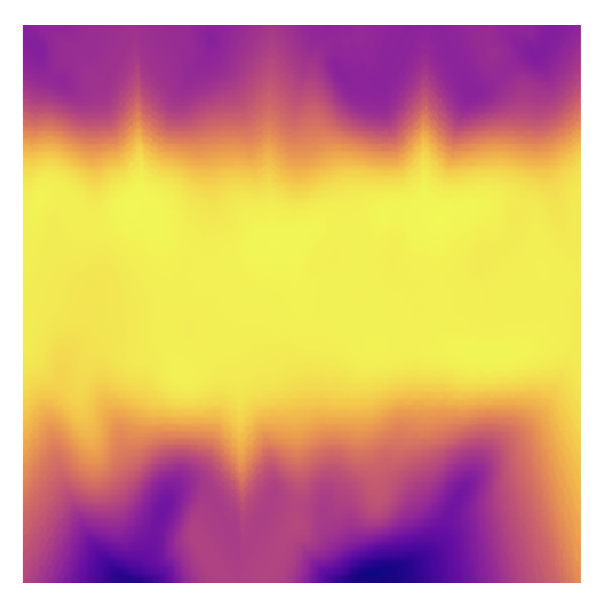
\includegraphics[width=0.9\linewidth]{figures/chapter-8/geopoth_goode.png}
        \caption{ Geopotential height raster data as Sinusoidal Sanson Flamsteed projected}
        \label{fig:sinu_geopoth_raster}
    \end{minipage}\hfill
    \begin{minipage}{0.30\textwidth}
        \centering
        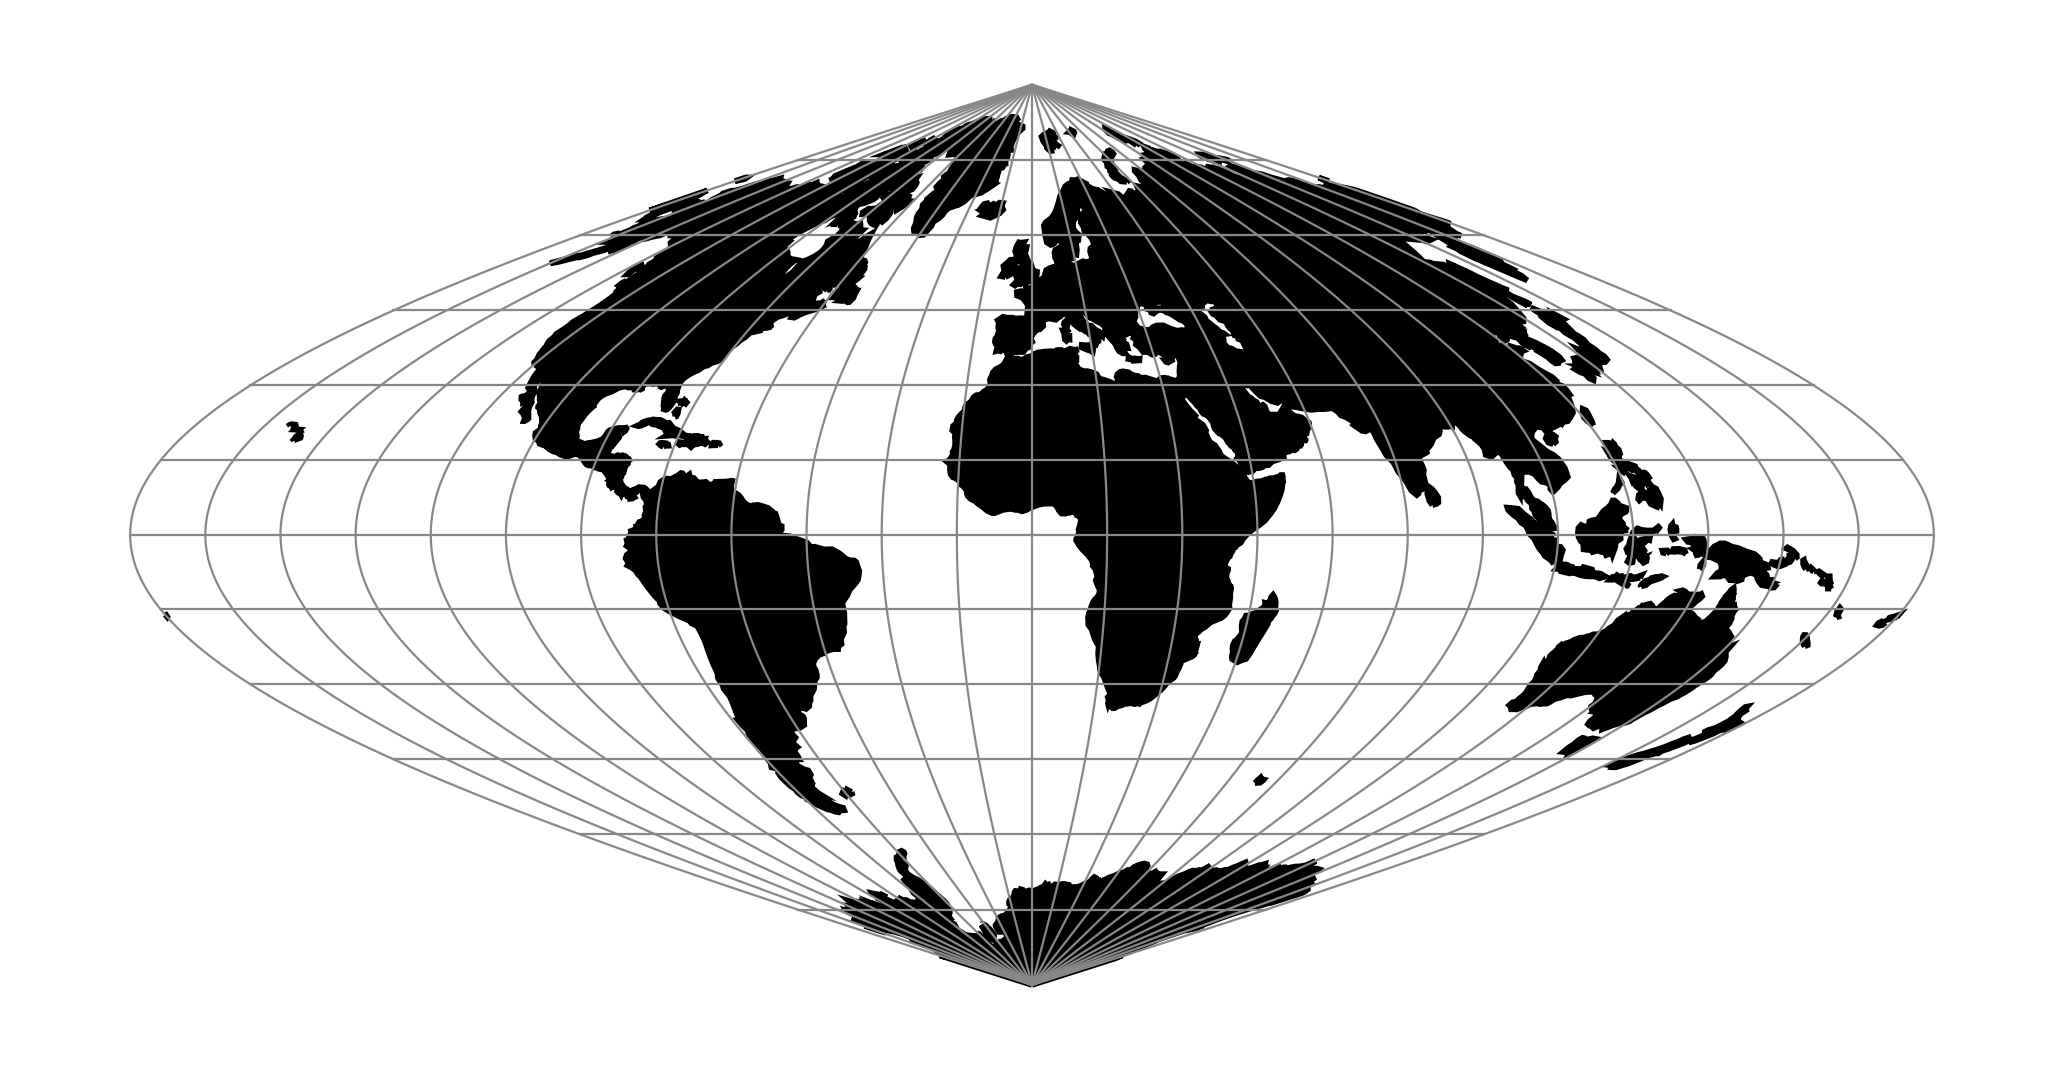
\includegraphics[width=0.9\linewidth]{figures/chapter-8/sinu.png}
        \caption{Sinusoidal Sanson Flamsteed (Source \cite{PROJ_SITE})}
        \label{fig:sinu_proj}
    \end{minipage}\hfill
    \begin{minipage}{0.30\textwidth}
        \centering
        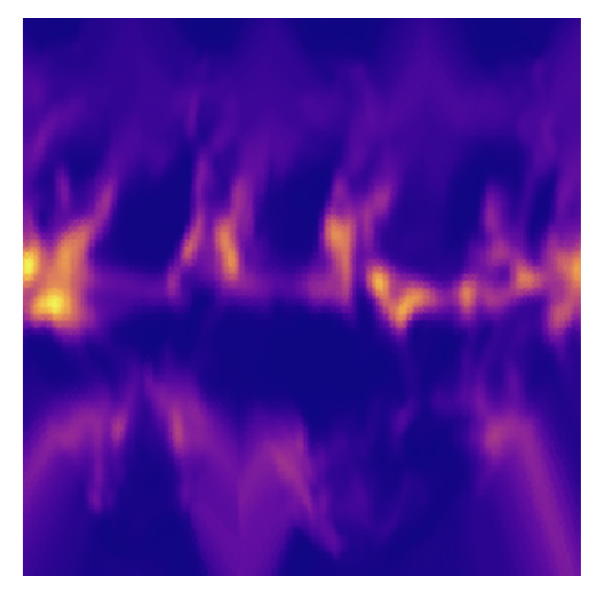
\includegraphics[width=0.9\linewidth]{figures/chapter-8/prect_goode.png}
        \caption{Precipitation raster data as Sinusoidal Sanson Flamsteed projected}
        \label{fig:sinu_prect_raster}
    \end{minipage}\hfill
\end{figure}


\begin{figure}[H]
    \centering
    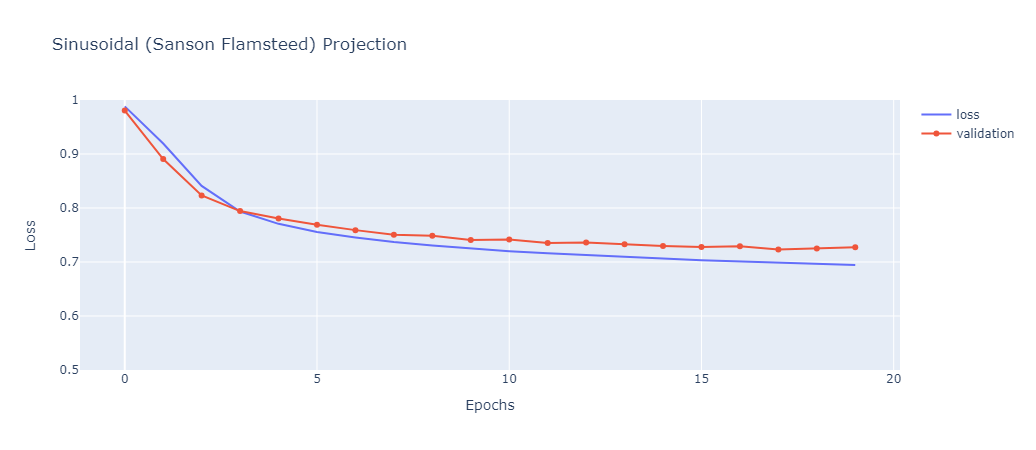
\includegraphics[width=1.0\linewidth]{figures/chapter-8/sinu_loss.png}
    \caption{Sinusoidal Sanson Flamsteed: Averaged training loss of models  }
    \label{fig:sinu_loss}
\end{figure}


\subsection{Results and Observations}
\begin{itemize}
    \item The Figures \ref{fig:robin_loss} \ref{fig:goode_loss} \ref{fig:sinu_loss} depict the training loss for the 3 of the 4 pseudocylindrical projections, the training and the validation loss value starts from a very high value of 1. All of the models are trended towards the overfitting trend,
          but the loss values are not decreasing as compared to the cylindrical projections.
    \item The overfitting trends are occuring in the robinson projection at epoch 8.
    \item The trend of overfitting in goode homolosine projected data is at epoch 7 and for the sinusoidal model it is on the 4th epoch.
    \item For the loximuthal projection the loss value is 0.690 and the validation loss is 0.716, even this projection is subjected to overfitting.
    \item It is the same phenomenon which was happening in the cylindrical projections when the data is spread on the whole raster, the model is overfitting, this projection is very much similar to robinson projection.
    \item The results in the Table ~\ref{pseudo_cylindrical_results_table} for predictions as compared to cylindrical projections is worse.
\end{itemize}
\begin{table}[ht]
    \centering
    \caption{Summary of Pseudocylindrical Projection Model Performance}
    \label{pseudo_cylindrical_results_table}
    \renewcommand{\arraystretch}{1.2} % Adjusts the row height
    \begin{tabular}{|l|c|c|c|c|c|}
        \hline
        \rowcolor[gray]{0.9}
        \textbf{\emph{Projection}}   & \textbf{\emph{\# Epochs}} & \textbf{\emph{MAE}} & \textbf{\emph{Validation MAE}} \\ \hline
        Robinson                     & 20                        & 0.617               & 0.627                          \\ \hline
        Interrupted Goode Homolosine & 20                        & 0.606               & 0.617                          \\ \hline
        Sinusoidal Sanson Flamsteed  & 20                        & 0.624               & 0.641                          \\ \hline
        Loximuthal                   & 20                        & 0.628               & 0.636                          \\ \hline
    \end{tabular}
\end{table}

\clearpage
\newpage
\section{Experiments: Conic Projections}
The selected conic projections for the experimentation are mentioned below:
\begin{itemize}
    \item Lambert Equal Area Conic
    \item Albers Equal Area
    \item Vitkovsky I
    \item Lambert Conformal Conic Alternative
\end{itemize}


% \subsection{Lambert Equal Area Conic}
\begin{figure}[H]
    \centering
    \begin{minipage}{0.30\textwidth}
        \centering
        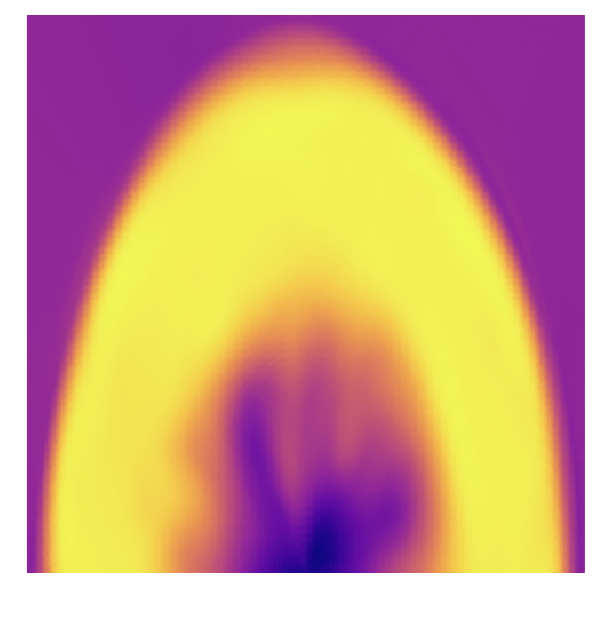
\includegraphics[width=0.9\linewidth]{figures/chapter-8/geopoth_leac.png}
        \caption{ Geopotential height raster data as Lambert Equal Area Conic projected}
        \label{fig:leac_geopoth_raster}
    \end{minipage}\hfill
    \begin{minipage}{0.30\textwidth}
        \centering
        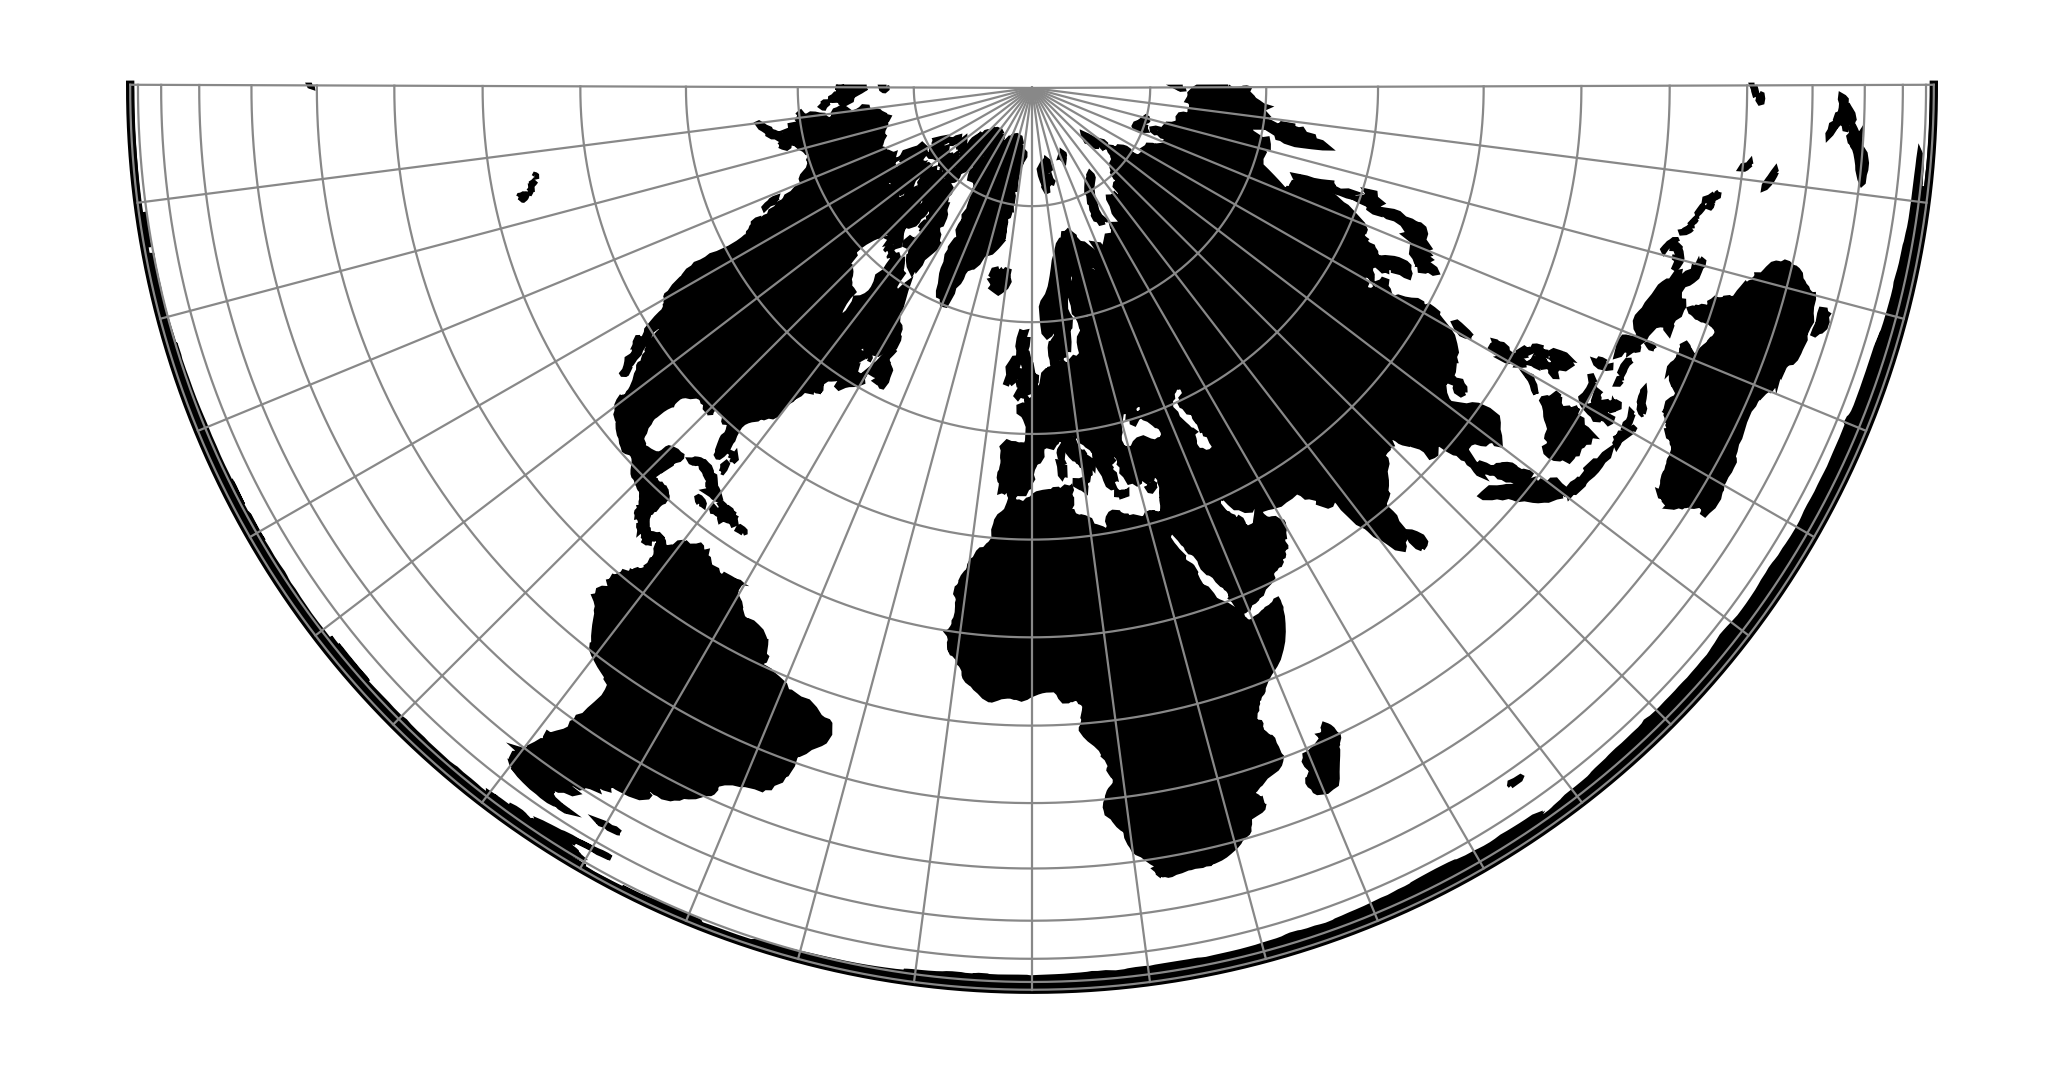
\includegraphics[width=0.9\linewidth]{figures/chapter-8/leac.png}
        \caption{Lambert Equal Area Conic (Source \cite{PROJ_SITE})}
        \label{fig:leac_proj}
    \end{minipage}\hfill
    \begin{minipage}{0.30\textwidth}
        \centering
        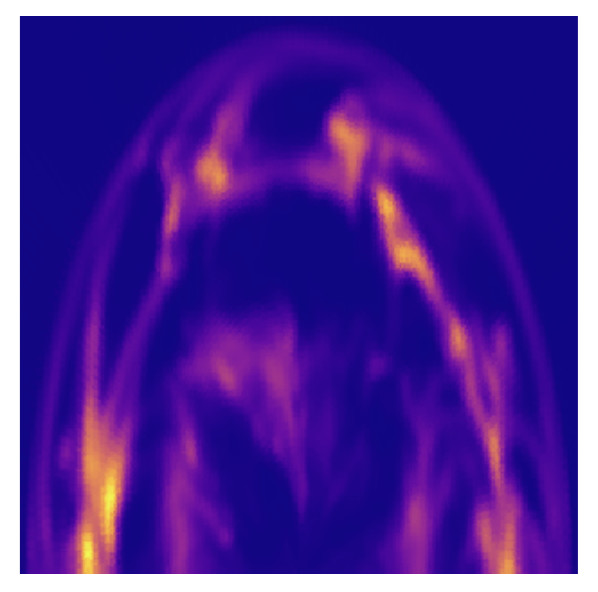
\includegraphics[width=0.9\linewidth]{figures/chapter-8/prect_leac.png}
        \caption{Precipitation raster data as Lambert Equal Area Conic projected}
        \label{fig:leac_prect_raster}
    \end{minipage}\hfill
\end{figure}
% \subsection{Albers Equal Area}
% \begin{figure}[h]
%     \centering
%     \begin{minipage}{0.30\textwidth}
%         \centering
%         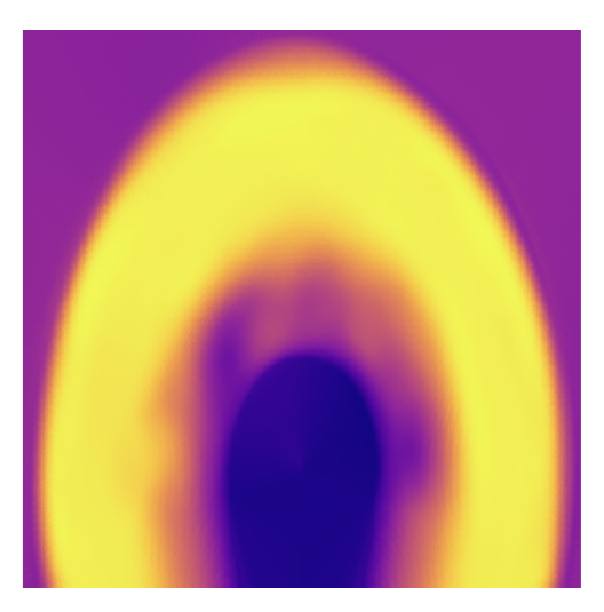
\includegraphics[width=0.9\linewidth]{figures/chapter-8/geopoth_aea.png}
%         \caption{ Geopotential height raster data as Albers Equal Area projected}
%         \label{fig:aea_geopoth_raster}
%     \end{minipage}\hfill
%     \begin{minipage}{0.30\textwidth}
%         \centering
%         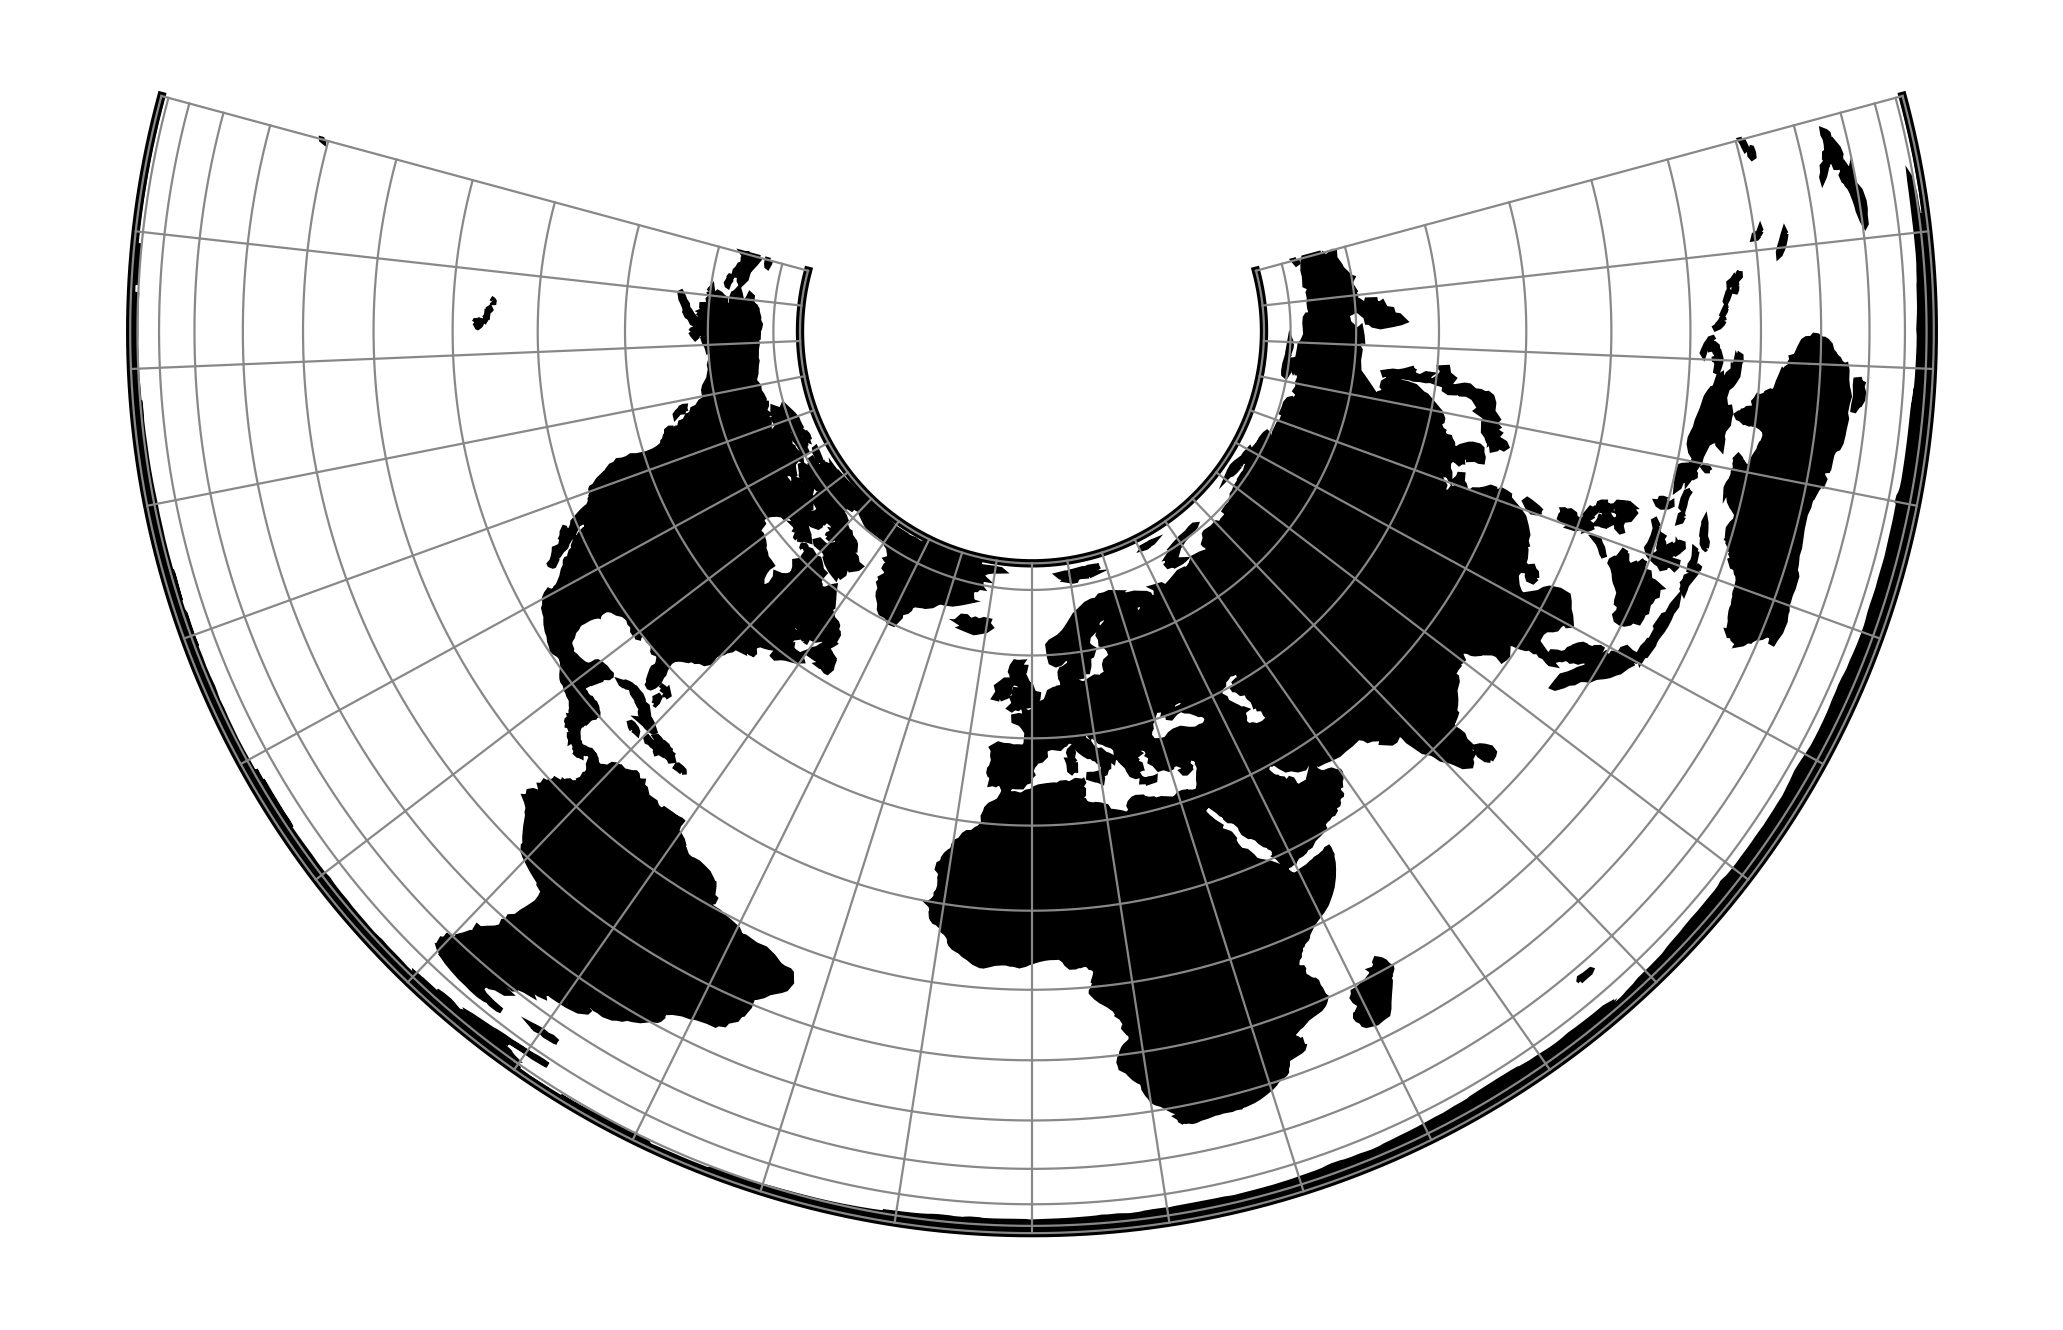
\includegraphics[width=0.9\linewidth]{figures/chapter-8/aea.png}
%         \caption{Albers Equal Area (Source \cite{PROJ_SITE})}
%         \label{fig:aea_proj}
%     \end{minipage}\hfill
%     \begin{minipage}{0.30\textwidth}
%         \centering
%         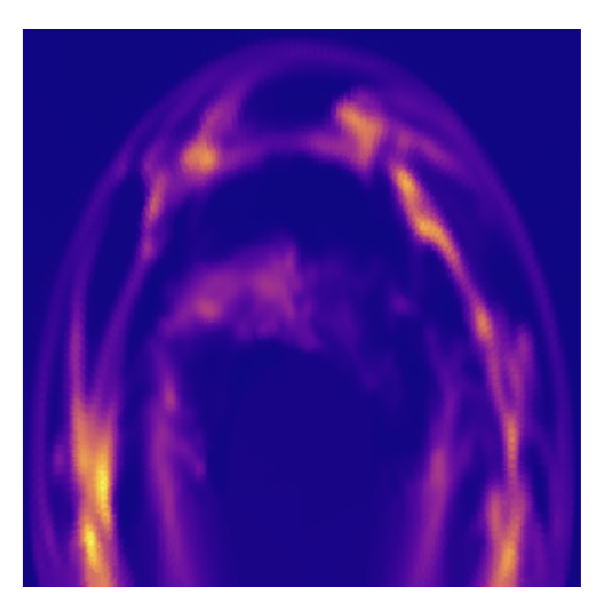
\includegraphics[width=0.9\linewidth]{figures/chapter-8/prect_aea.png}
%         \caption{Precipitation raster data as Albers Equal Area projected}
%         \label{fig:aea_prect_raster}
%     \end{minipage}\hfill
% \end{figure}
% \newpage
% \subsection{Vitkovsky I}
% \begin{figure}[h]
%     \centering
%     \begin{minipage}{0.30\textwidth}
%         \centering
%         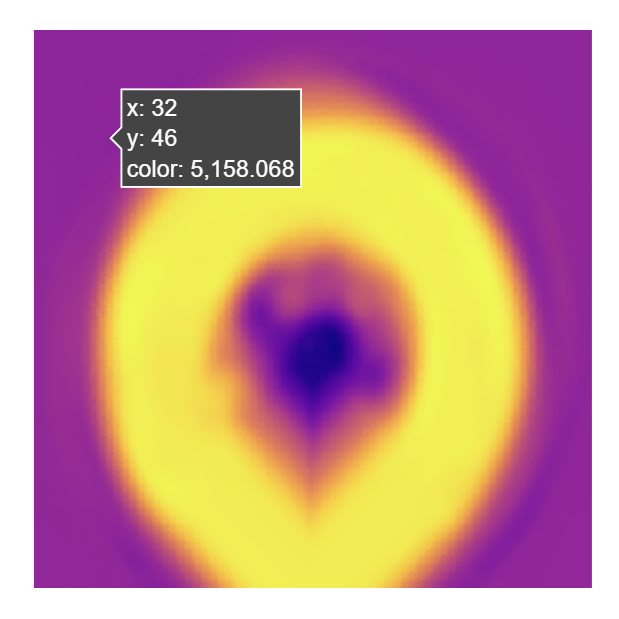
\includegraphics[width=0.9\linewidth]{figures/chapter-8/geopoth_vitk.png}
%         \caption{ Geopotential height raster data as Vitkovsky I projected}
%         \label{fig:vitk_geopoth_raster}
%     \end{minipage}\hfill
%     \begin{minipage}{0.30\textwidth}
%         \centering
%         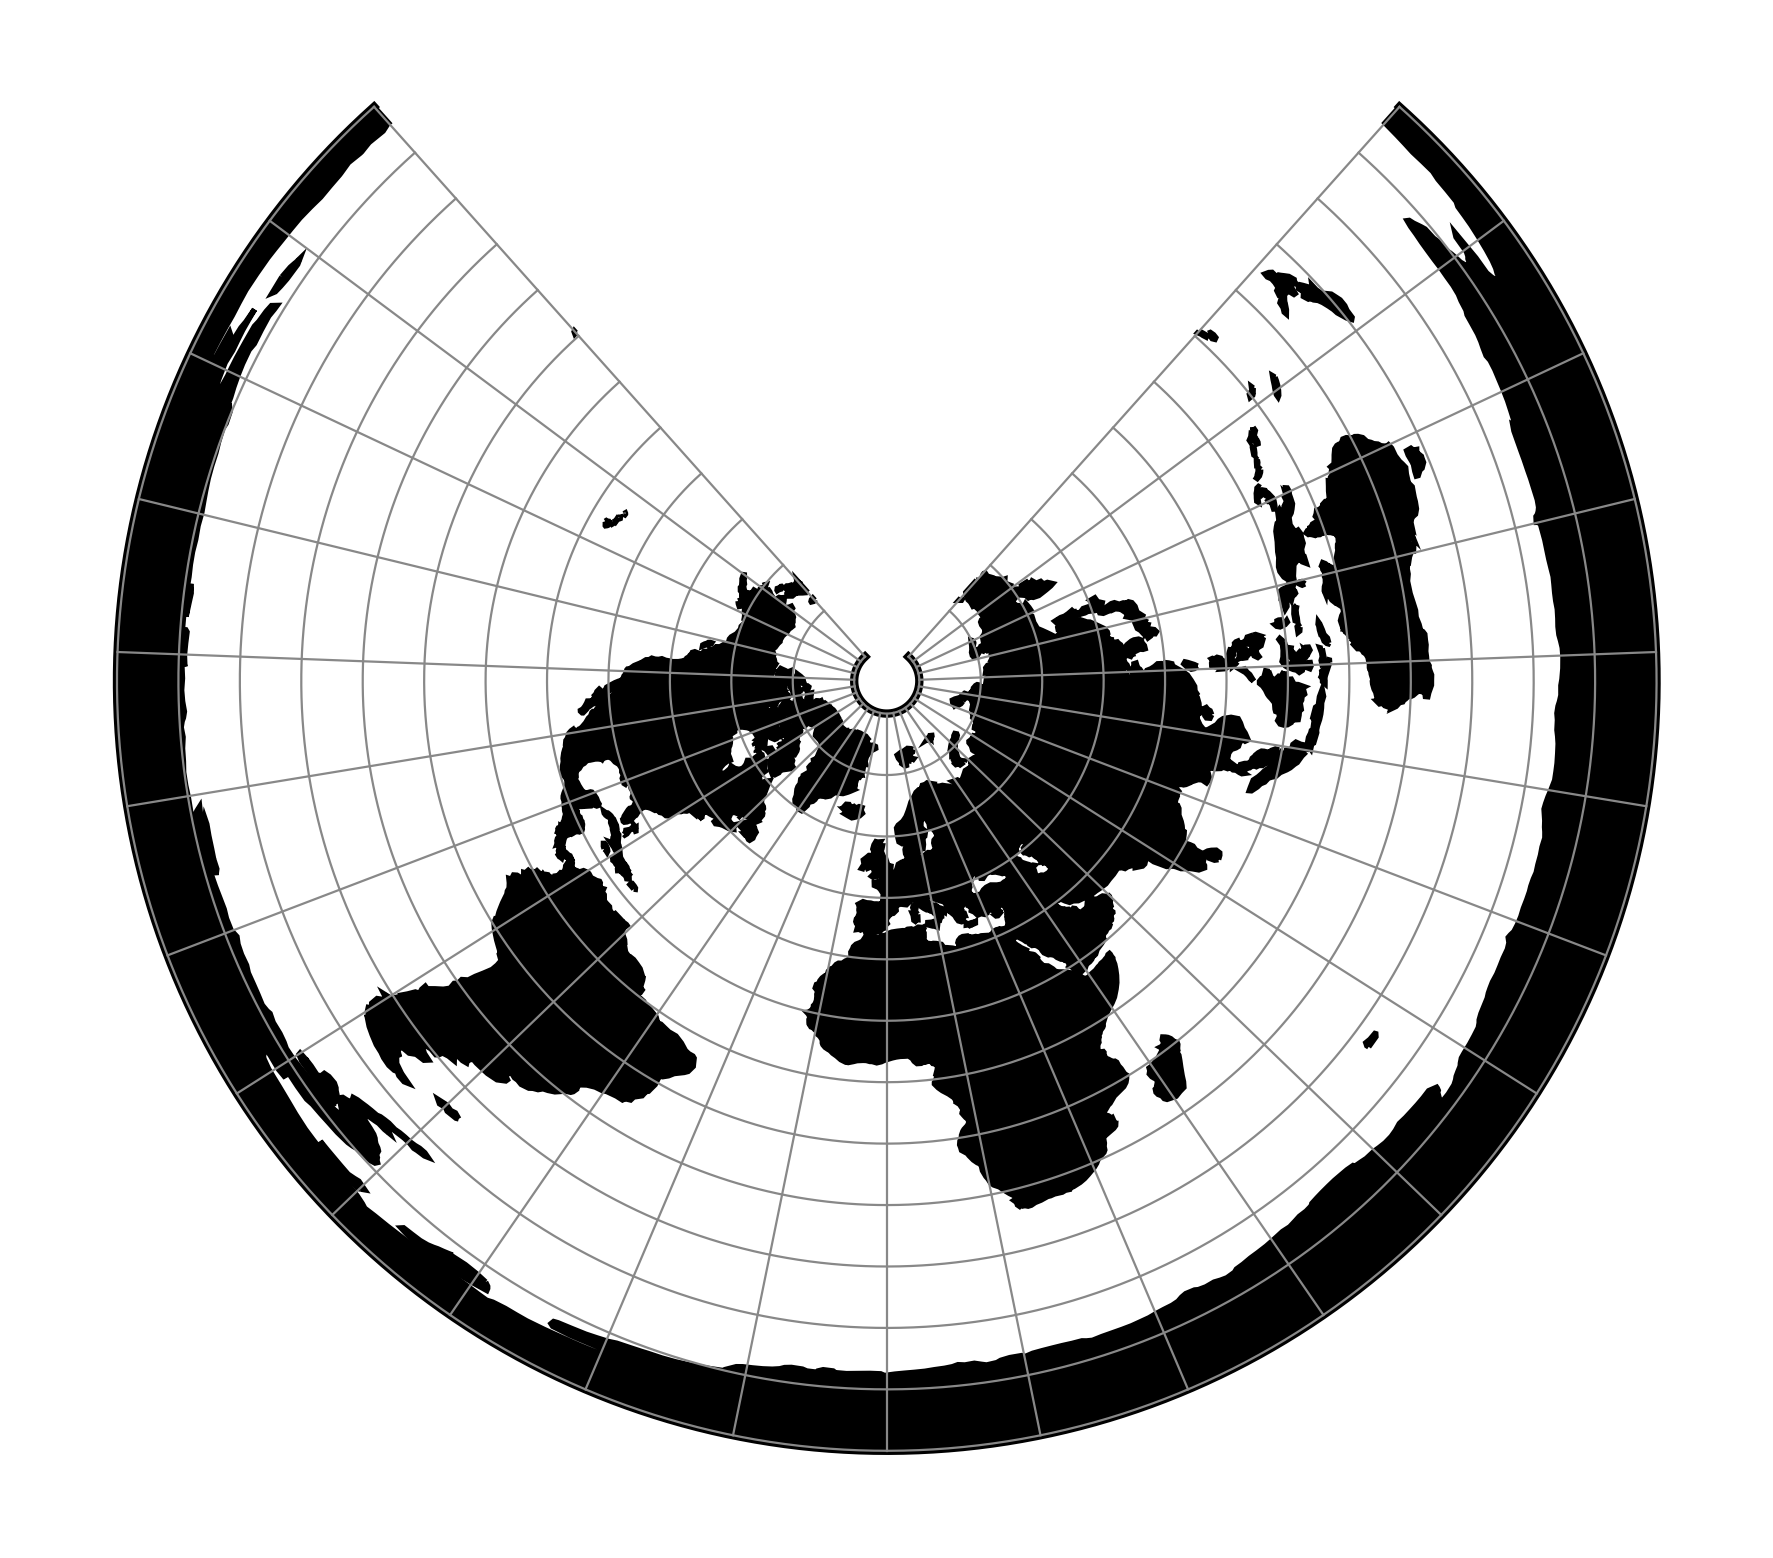
\includegraphics[width=0.9\linewidth]{figures/chapter-8/vitk1.png}
%         \caption{Vitkovsky I (Source \cite{PROJ_SITE})}
%         \label{fig:vitk_proj}
%     \end{minipage}\hfill
%     \begin{minipage}{0.30\textwidth}
%         \centering
%         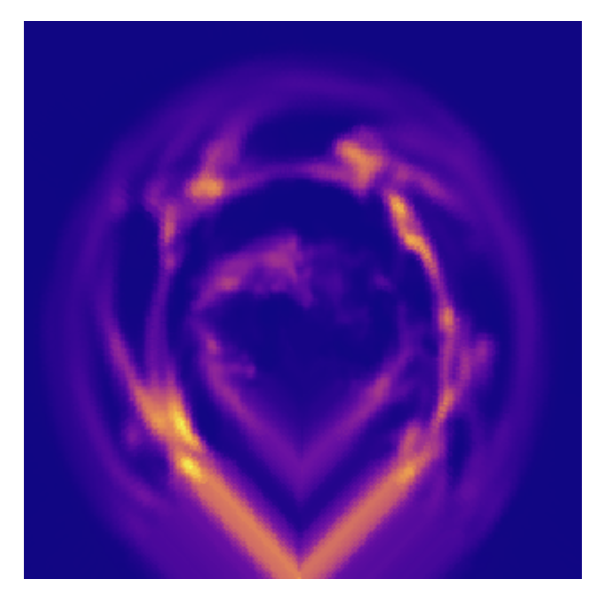
\includegraphics[width=0.9\linewidth]{figures/chapter-8/prect_vitk.png}
%         \caption{Precipitation raster data as Vitkovsky I projected}
%         \label{fig:vitk_prect_raster}
%     \end{minipage}\hfill
% \end{figure}
% \subsection{Lambert Conformal Conic Alternative}
% \begin{figure}[h]
%     \centering
%     \begin{minipage}{0.30\textwidth}
%         \centering
%         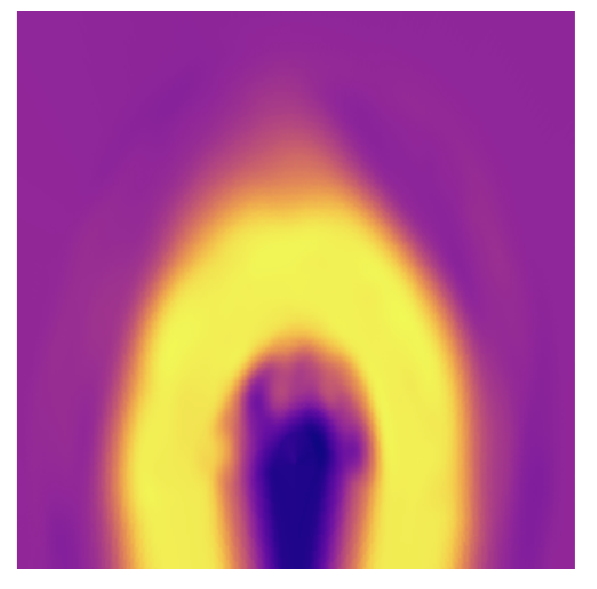
\includegraphics[width=0.9\linewidth]{figures/chapter-8/geopoth_lcca.png}
%         \caption{ Geopotential height raster data as Lambert Conformal Conic Alternative projected}
%         \label{fig:lcca_geopoth_raster}
%     \end{minipage}\hfill
%     \begin{minipage}{0.30\textwidth}
%         \centering
%         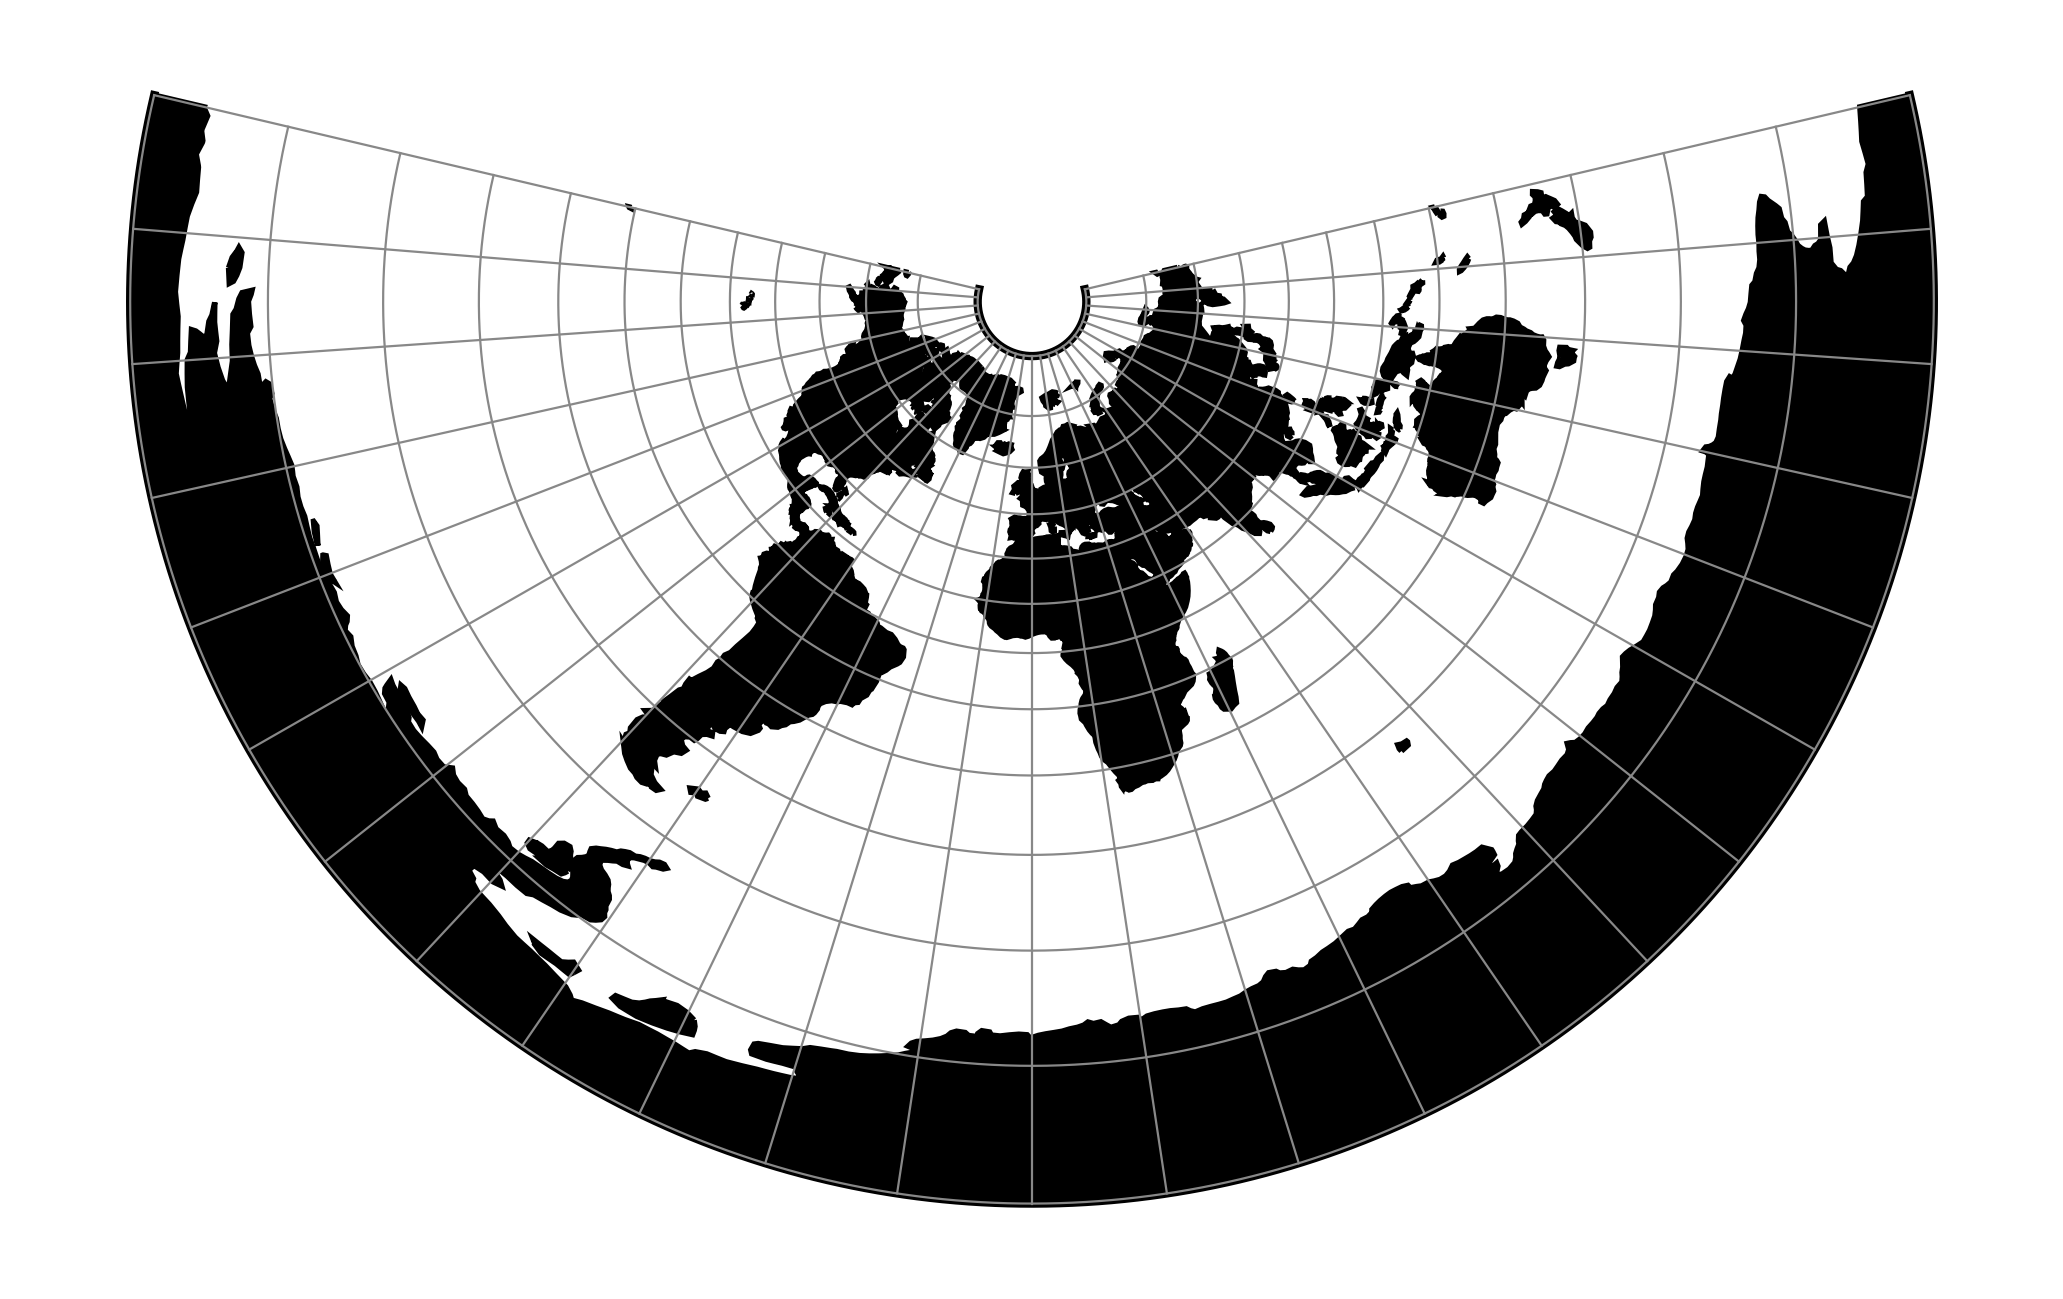
\includegraphics[width=0.9\linewidth]{figures/chapter-8/lcca.png}
%         \caption{Lambert Conformal Conic Alternative (Source \cite{PROJ_SITE})}
%         \label{fig:lcca_proj}
%     \end{minipage}\hfill
%     \begin{minipage}{0.30\textwidth}
%         \centering
%         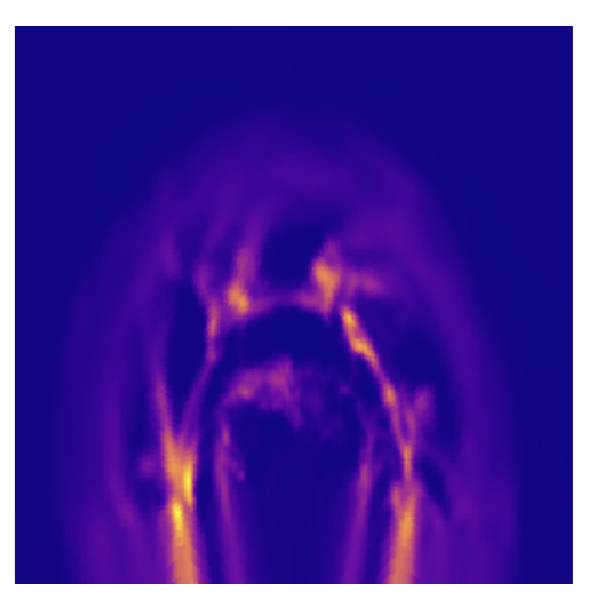
\includegraphics[width=0.9\linewidth]{figures/chapter-8/prect_lcca.png}
%         \caption{Precipitation raster data as Lambert Conformal Conic Alternative projected}
%         \label{fig:lcca_prect_raster}
%     \end{minipage}\hfill
% \end{figure}

\subsection{Results and Observations}
\begin{itemize}
    \item The conic projections are not well suited for the representation of the global data, as the areas around the poles are either stretched or squeezed too much.
    \item The north pole data for some of the conic projections loss the neighborhood correlation as well.
    \item The training and the validation loss for the selected conic projections is depited in the table ~\ref{conic_results_table}, showing that model is not able to learn for these experiments.
    \item The metric to depict prediction is depicted in the ~\ref{conic_results_table}.
\end{itemize}
\begin{table}[ht]
    \centering
    \caption{Summary of Conic Projection Model Performance}
    \label{conic_results_table}
    \renewcommand{\arraystretch}{1.2} % Adjusts the row height
    \begin{tabular}{|l|c|c|c|c|}
        \hline
        \rowcolor[gray]{0.9}
        \textbf{\emph{Projection}}          & \textbf{\emph{\# Epochs}} & \textbf{\emph{MAE}} & \textbf{\emph{Validation MAE}} \\ \hline
        Lambert Equal Area Conic            & 20                        & 0.597               & 0.608                          \\ \hline
        Albers Equal Area                   & 20                        & 0.644               & 0.656                          \\ \hline
        Vitkovsky I                         & 20                        & 0.657               & 0.664                          \\ \hline
        Lambert Conformal Conic Alternative & 20                        & 0.670               & 0.674                          \\ \hline
    \end{tabular}
\end{table}

\clearpage
\newpage
\section{Planar Projections}

\subsubsection*{Lambert Azimuthal Equal Area}
\begin{figure}[h]
    \centering
    \begin{minipage}{0.30\textwidth}
        \centering
        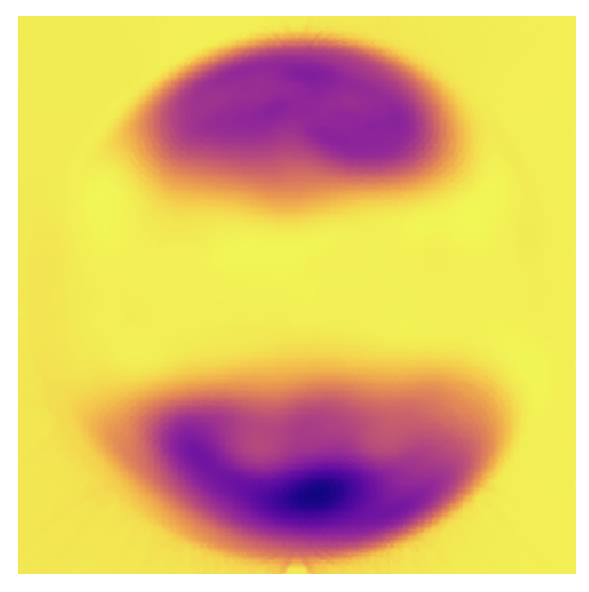
\includegraphics[width=0.9\linewidth]{figures/chapter-8/geopoth_laea.png}
        \caption{ Geopotential height raster data as Lambert Azimuthal Equal Area projected}
        \label{fig:laea_geopoth_raster}
    \end{minipage}\hfill
    \begin{minipage}{0.30\textwidth}
        \centering
        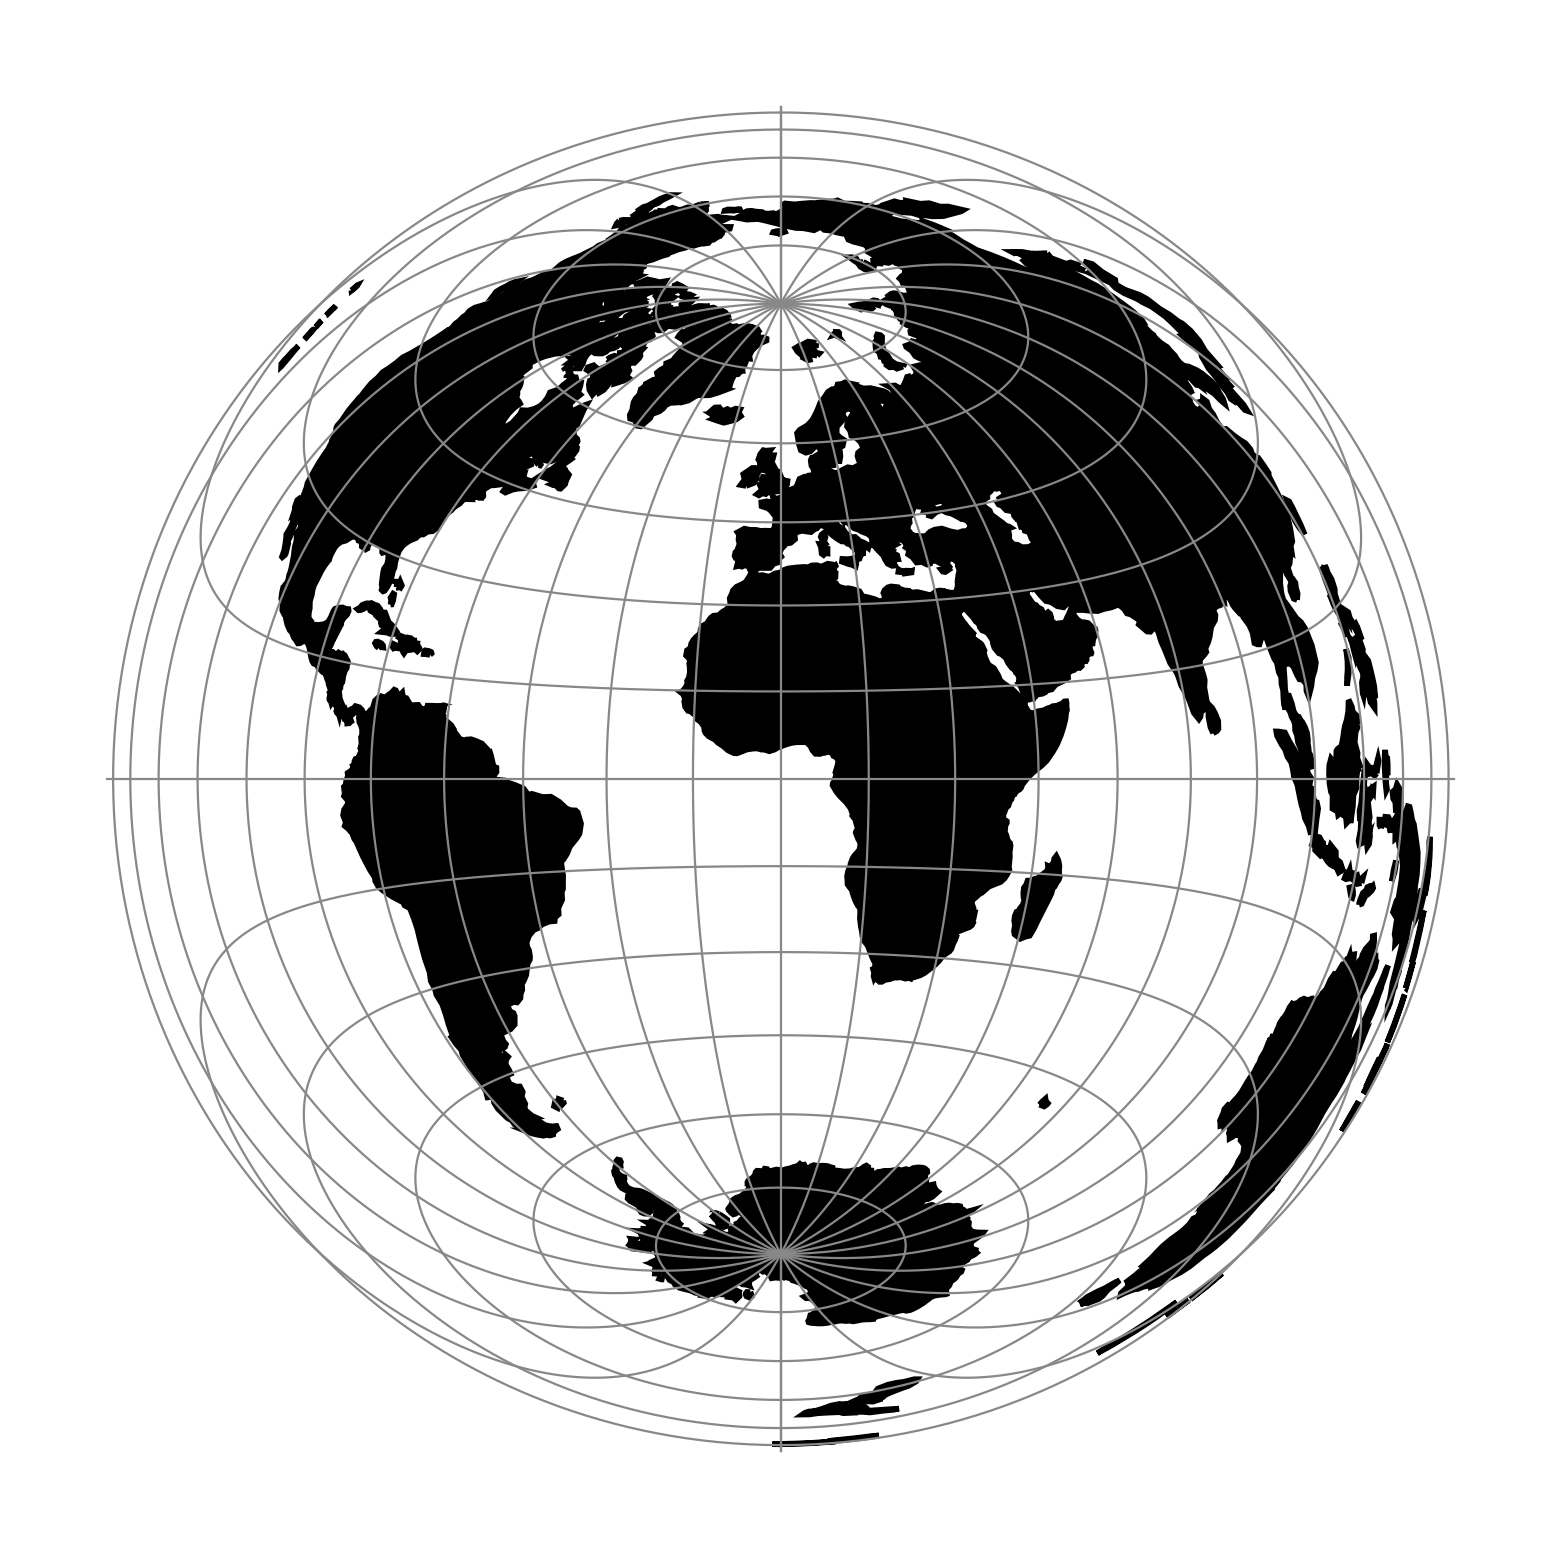
\includegraphics[width=0.9\linewidth]{figures/chapter-8/laea.png}
        \caption{Lambert Azimuthal Equal Area (Source \cite{PROJ_SITE})}
        \label{fig:laea_proj}
    \end{minipage}\hfill
    \begin{minipage}{0.30\textwidth}
        \centering
        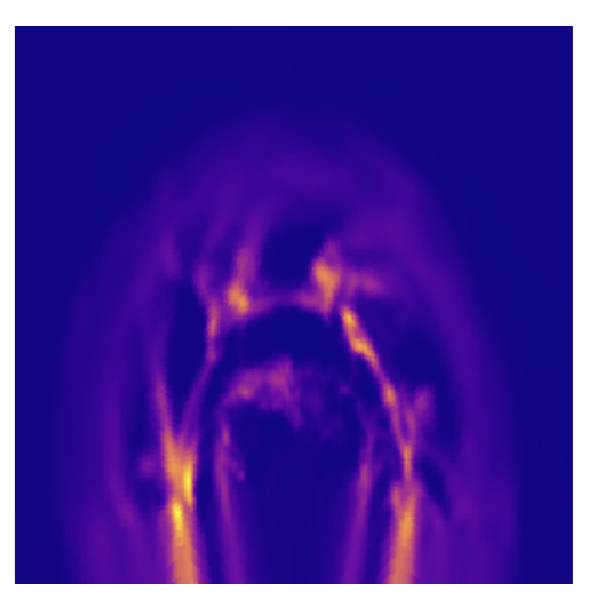
\includegraphics[width=0.9\linewidth]{figures/chapter-8/prect_lcca.png}
        \caption{Precipitation raster data as Lambert Azimuthal Equal Area projected}
        \label{fig:laea_prect_raster}
    \end{minipage}\hfill
\end{figure}

\subsubsection*{Wagner VII}
\begin{figure}[h]
    \centering
    \begin{minipage}{0.30\textwidth}
        \centering
        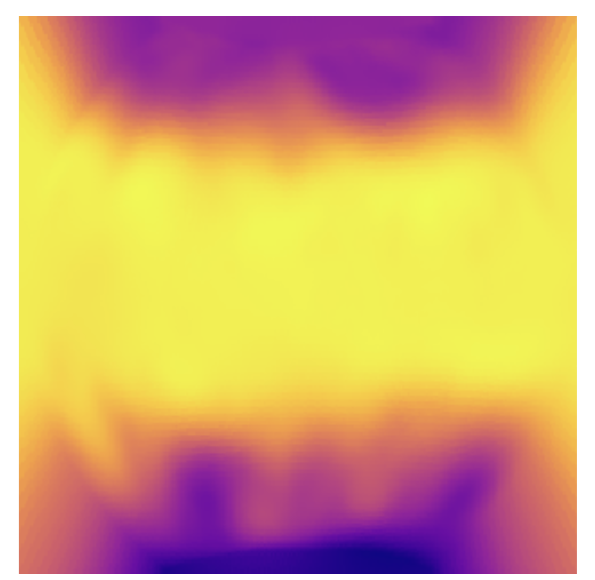
\includegraphics[width=0.9\linewidth]{figures/chapter-8/geopoth_wag.png}
        \caption{ Geopotential height raster data as Wagner VII projected}
        \label{fig:wag_geopoth_raster}
    \end{minipage}\hfill
    \begin{minipage}{0.30\textwidth}
        \centering
        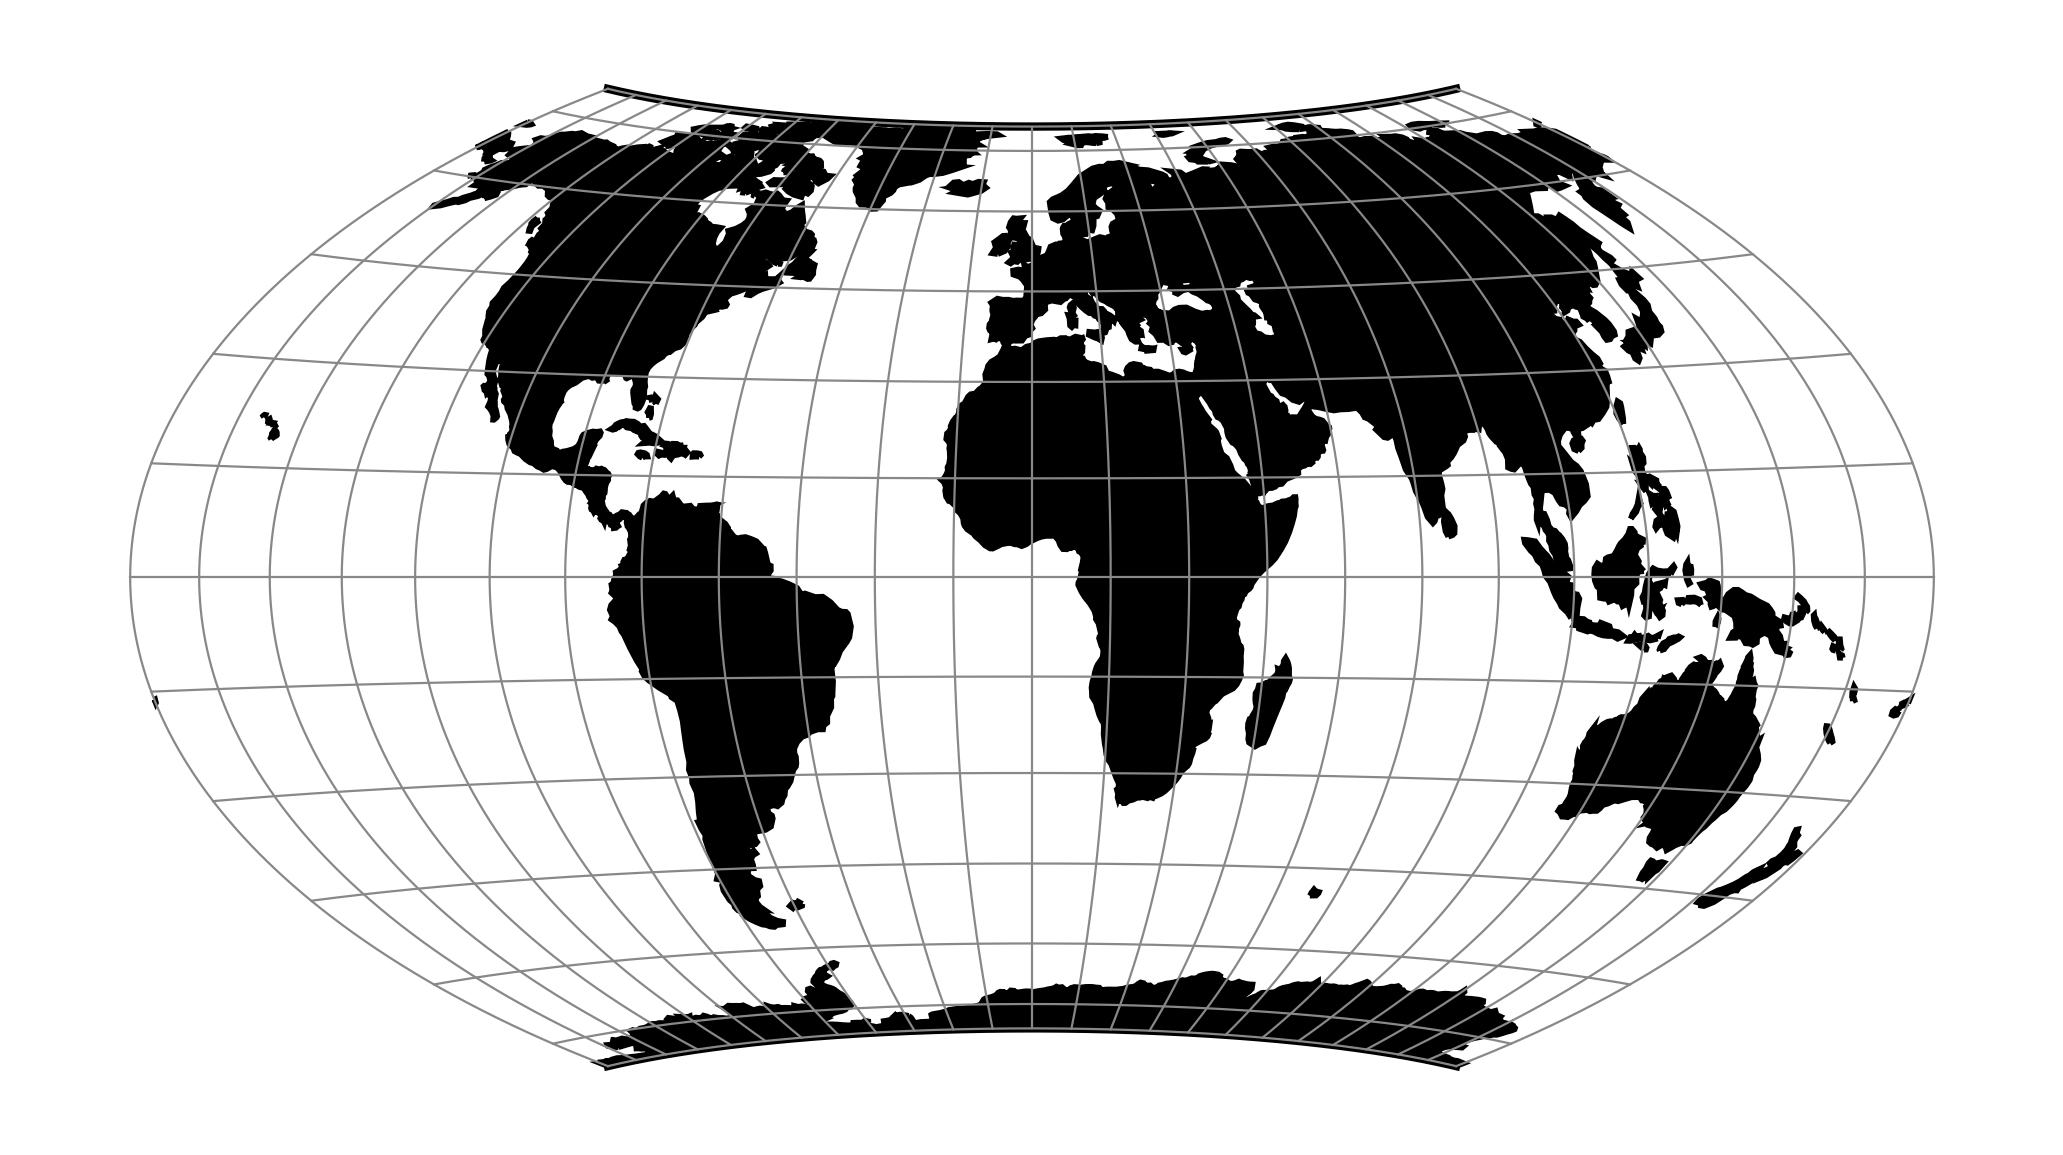
\includegraphics[width=0.9\linewidth]{figures/chapter-8/wag7.png}
        \caption{Wagner VII (Source \cite{PROJ_SITE})}
        \label{fig:wag_proj}
    \end{minipage}\hfill
    \begin{minipage}{0.30\textwidth}
        \centering
        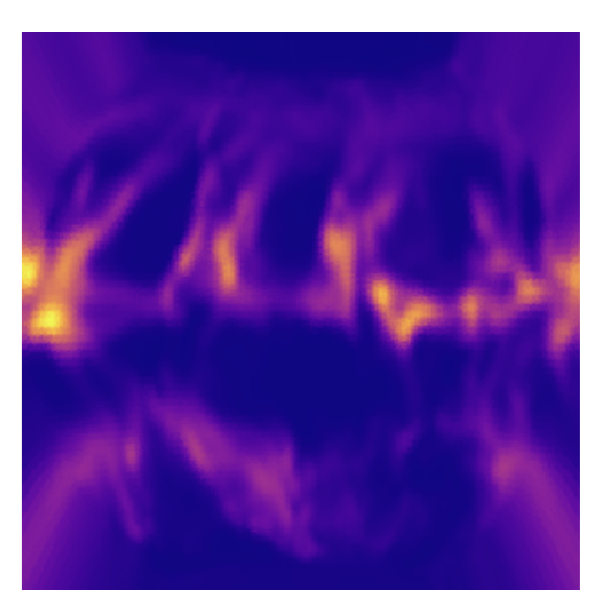
\includegraphics[width=0.9\linewidth]{figures/chapter-8/prect_wag.png}
        \caption{Precipitation raster data as Wagner VII projected}
        \label{fig:wag_prect_raster}
    \end{minipage}\hfill
\end{figure}

\subsection{Results}
\begin{table}[ht]
    \centering
    \caption{Summary of Model Performance}
    \label{planner_results_table}
    \renewcommand{\arraystretch}{1.2} % Adjusts the row height
    \begin{tabular}{|l|c|c|c|c|c|}
        \hline
        \rowcolor[gray]{0.9}
        \textbf{\emph{Project Name}} & \textbf{\emph{\# Epochs}} & \textbf{\emph{MAE}} & \textbf{\emph{Validation MAE}} & \textbf{\emph{MAPE}} & \textbf{\emph{Validation MAPE}} \\ \hline
        Project 1                    & 50                        & 0.05                & 0.06                           & 5\%                  & 6\%                             \\ \hline
        Project 2                    & 30                        & 0.04                & 0.05                           & 4\%                  & 5\%                             \\ \hline
        Project 3                    & 100                       & 0.03                & 0.04                           & 3\%                  & 4\%                             \\ \hline
    \end{tabular}
\end{table}



The experiments performed provides us the valauable insights for the usage of different types of map projections. Even though there are various map projections that could be used for the experimentation but the underlying
distortions by them will be effecting the analysis. Now we will conclude and propose the future endeavour for the search of a better Earth model for the geospatial analysis.